\documentclass[a4paper,12pt]{article}

\usepackage{cmap}
\usepackage[T2A]{fontenc}
\usepackage[utf8]{inputenc}
\usepackage[english,russian]{babel}
\usepackage[left=2cm,right=1.5cm,top=2cm,bottom=2cm]{geometry}
\tolerance=1000
\setlength{\emergencystretch}{3em}

\usepackage{amsmath,amssymb,amstext,amsfonts,amsthm}
\usepackage{mathtools}
\usepackage{booktabs,longtable,array}
\usepackage{graphicx}
\usepackage{placeins}
\graphicspath{{images/}{myself/images/}}
\usepackage{indentfirst}
\usepackage{stmaryrd}

\newcommand{\N}{\mathbb{N}}
\newcommand{\Z}{\mathbb{Z}}
\newcommand{\R}{\mathbb{R}}
\newcommand{\Q}{\mathbb{Q}}
\newcommand{\CC}{\mathbb{C}}
\newcommand{\Bo}{\mathring{B}}
\renewcommand{\phi}{\varphi}
\renewcommand{\epsilon}{\varepsilon}
\renewcommand{\emptyset}{\varnothing}
\renewcommand{\Gamma}{\varGamma}
\DeclareMathOperator*{\lowlim}{\underline{lim}}
\DeclareMathOperator*{\uplim}{\overline{lim}}
\DeclareMathOperator*{\Img}{Im}
\DeclareMathOperator*{\esup}{ess\ sup}

\theoremstyle{plain}
\newtheorem*{theorem}{Теорема}
\newtheorem*{corollary}{Следствие}
\newtheorem*{statement}{Утверждение}
\newtheorem*{lemma}{Лемма}
\newtheorem*{proposition}{Утверждение}
\theoremstyle{definition}
\newtheorem*{definition}{Определение}
\newtheorem*{example}{Пример}
\theoremstyle{remark}
\newtheorem*{remark}{Замечание}

\usepackage{titlesec}
%\titleformat{\section}{\LARGE\bfseries}{\thesection}{1em}{}
%\titleformat{\subsection}{\Large\bfseries}{\thesubsection}{1em}{}
%\titleformat{\subsubsection}{\large\bfseries}{\thesubsubsection}{1em}{}
\numberwithin{equation}{section}
\newcommand{\tab}[1][.5cm]{\hspace*{#1}}

\usepackage{xcolor}
\definecolor{linkcolor}{HTML}{225ae2}
\definecolor{urlcolor}{HTML}{225ae2}
\usepackage[unicode]{hyperref}
\hypersetup{
  pdfstartview=FitH,
  linkcolor=linkcolor,
  urlcolor=urlcolor,
  citecolor=linkcolor,
  colorlinks=true
}

\newcommand{\Reg}{\operatorname{Reg}}
\newcommand{\ind}{\mathbf{1}}

% Замените название и впишите имя автора.
\title{Адаптивное агрегирование прогнозов специализированных экспертов}
\author{Е.А. Цыбулин} % Ваше имя и фамилия.
\date{\today} % Для документа без даты используйте \date{}.

\begin{document}
\maketitle

% При необходимости раскомментируйте аннотацию.
% \begin{abstract}
% Краткое описание задачи и основных результатов доклада.
% \end{abstract}

%\tableofcontents
%\newpage

% Ниже начинается ваш текст. Названия разделов можно свободно менять.
% \section{Введение}
% \label{sec:introduction}
% \begin{enumerate}
%   \item Prediction with expert advice
%   \item Кто такие эксперты?
%   \item Природа временного ряда
%   \item Прогнозировать можно потребление электроэнегии или спрос на товар, как в данной работе.
%   \item Оценка прогноза - loss
%   \item Оценка прогноза - regret
%   \item Используемые методы прогнозирования значения временного ряда: Ridge regression, Lasso regression, Bayesian Ridge regression, Random Forest regression, Gradient Boosting regression.
%   \item Специализированные, или спящие, эксперты -> специализированные стратегии
%   \item Преимущества: можно в рандомный момент времени добавлять новых экспертов, а также допустимы пропуски значений.
% \end{enumerate} 

\section{Стандартная постановка задачи и основные определения}
\label{sec:problem}
Рассматривается задача прогнозирования временного ряда с использованием экспертных стратегий (\textit{prediction with expert advice}). \textit{Временной ряд} $y = (y_1, y_2, \dots)$ представляет собой последовательность элементов некоторого множества $\mathcal{Y}$, называемых исходами. 
В рамках данной теории строятся алгоритмы, называемые \textit{смешивающими прогнозирующими алгоритмами (ПА)}, объединяющие предсказания следующего исхода различных методов прогнозирования. 

Экспертные стратегии (далее — \textit{эксперты}) могут иметь совершенно разную природу — это могут быть некоторые правила, функции, алгоритмы, оценки специалистов и т.д. Каждый эксперт может быть эффективнее других на определённых участках ряда.

Классическая задача заключается в том, что в режиме онлайн на шагах $t = 1, 2, \dots$ генерируются исходы $y_1, y_2, \dots \in \mathcal{Y}$. 
В каждый момент времени $t \in \N$ смешивающий ПА, зная предыдущие исходы, а также предсказания $\gamma_t^i$, $i = 1, \dots, N$ из множества допустимых прогнозов $\mathcal{D}$ конечного числа экспертов из множества $I = \{1, \dots, N\}$, делает свой прогноз $\gamma_t \in \mathcal{D}$.
После того, как становится следующий исход $y_t$, каждый эксперт, а также смешивающий ПА оцениваются величиной потерь.

Потери на шаге $t$ равны значению \textit{функции потерь (лосс)}
\[\ell: \mathcal{D} \times \mathcal{Y} \to [0, +\infty)\]
на паре $(\gamma_t, y_t)$ для смешивающего ПА и на паре $(\gamma_t^i, y_t)$ — для эксперта $i$.
Примеры функций потерь:
\[\ell(\gamma, y) = \lambda_1 |\gamma - y|_+ + \lambda_2 |y - \gamma|_+,\]
где $|x|_+ := \max{(x, 0)}$,
\[\ell(\gamma, y) = (\gamma - y)^2, \quad \ell(\gamma, y) = \llbracket \gamma \neq y \rrbracket.\]
Также имеют место суммарные (кумулятивные) потери на отрезке $t = 1, \dots, T$:
\[L_T := \sum\limits_{t=1}^{T} \ell(\gamma_t, y_t), \quad L_T^i := \sum\limits_{t=1}^{T} \ell(\gamma_t^i, y_t).\]

Наша цель — получить смешивающий ПА, который выдаёт ответы, наиболее близкие к ответам наилучшего эксперта.
Поскольку происхождение исходов нам неизвестно (природа временного ряда необязательно имеет вероятностный характер, поэтому исходы могут иметь как стохастическую природу, так и детерминированную или вообще враждебную по отношению к прогнозирующему алгоритму), то нельзя определить понятие риска.
Основной гарантией эффективности алгоритма является \textit{регрет относительно лучшего фиксированного эксперта}:
\[R_T := L_T - \min\limits_{1 \leqslant i \leqslant N} L_T^i.\]


\section{Смешивание потерь}
Определим понятие вероятностного распределения на множестве $I = \{1, \dots, N\}$, которое представляет собой произвольный вектор $\bar{p_t} = (p^1, \dots, p^N)$, где $\sum\limits_{i=1}^{N}p^i = 1$, $p^i \geqslant 0$, $i = 1, \dots, N$. Множество всех вероятностных распределений будем обозначать $I^{\Delta}$.

Рассмотрим задачу смешивания потерь: пусть на каждом шаге известны только потери экспертов (конкретная функция потерь может отсутствовать). 
На каждом шаге $t = 1, 2, \dots$:
\begin{enumerate}
  \item смешивающий ПА находит вектор распределения экспертов $\bar{p_t} = (p^1, \dots, p^N) \in I^\Delta$;
  \item эксперты объявляют потери $\ell_t^i$, также пусть $\bar{\ell_t} = (\ell_t^1, \dots, \ell_t^N)$;
  \item смешивающий ПА подсчитывает свои потери $\ell_t = (\bar{p_t} \cdot \bar{\ell_t}) := \sum\limits_{i=1}^{N}p_t^i \cdot \ell_t^i$;
  \item смешивающий ПА пересчитывает вектор распределения.
\end{enumerate}
Предполагаем, что потери экспертов ограничены, например, $\ell_t^i \in [0,1] \ \forall t \in \N, \ \forall i \in \{1, \dots, N\}$.
Определим кумулятивные потери:
\[L_T = \sum\limits_{i=1}^{T} (\bar{p_t} \cdot \bar{\ell_t}), \quad L_T^i = \sum\limits_{i=1}^{T} \ell_t^i.\]

Задача смешивающего ПА заключается в подборе вектора распределения таким образом, что
\[R_T = L_T - \min\limits_{1 \leqslant i \leqslant N} L_T^i \to \min_{I^\Delta}.\]


\subsection{Экспоненциальное смешивание потерь}
Для решения задачи рассмотрим алгоритм $Hedge(\eta)$, который имеет входные параметры $\eta$ — параметр обучения и начальный набор весов экспертов $(w_1^1, \dots, w_1^N)$.
Пусть веса экспертов в начальный момент времени определены равномерным распределением, то есть $w_1^i = \frac{1}{N}$, $\forall i \in I$.
Для моментов времени $t = 1, 2, \dots$:
\begin{itemize}
  \item алгоритм вычисляет $\bar{p_t} = \frac{\bar{w_t}}{\sum\limits_{i=1}^{N}w_t^i}$ — вектор распределения экспертов;
  \item эксперты объявляют свои потери $\ell_t^i$, также пусть $\bar{\ell_t} = (\ell_t^1, \dots, \ell_t^N)$;
  \item алгоритм подсчитывает свои потери $\ell_t = (\bar{p_t} \cdot \bar{\ell_t}) := \sum\limits_{i=1}^{N}p_t^i \cdot \ell_t^i$;
  \item алгоритм пересчитывает веса экспертов $$w_{t+1}^i = w_t^i \cdot \exp\left(-\eta \ell_t^i\right).$$
\end{itemize}
Определим кумулятивные потери:
\[H_T = \sum\limits_{s=1}^{T} \ell_s, \quad L_T^i = \sum\limits_{s=1}^{T} \ell_s^i.\]
Легко видеть, что
\[w_t^i = w_1^i \cdot \exp\left(-\eta L_{t-1}^i\right).\]

Введём следующее понятие смешанной потери алгоритма:
\[m_t := -\frac{1}{\eta} \ln \left(\sum\limits_{i=1}^{N} p_t^i \cdot \exp \left(-\eta \ell_t^i\right)\right).\]
Очевидным образом определяются кумулятивные смешанные потери:
\[M_T := \sum\limits_{t=1}^{T} m_t.\]
Определим $W_t = \sum\limits_{i=1}^{N}w_t^i$ для всех $t$, тогда из определения следует, что $p_t^i = \frac{w_t^i}{W_t}$.

\begin{lemma}[Представление кумулятивных смешанных потерь]
Для любого $T \geqslant 1$ выполнено
\begin{equation}
\label{eq:mix-loss-potential}
M_T = -\frac{1}{\eta}\ln W_{T+1}
    = -\frac{1}{\eta}\ln\left(
        \sum_{i=1}^{N} w_1^i \exp\left(-\eta L_T^i\right)
      \right).
\end{equation}
\end{lemma}

\begin{proof}
По правилу обновления весов
\[
\sum_{i=1}^{N} p_t^i \exp\left(-\eta\ell_t^i\right)
= \frac{1}{W_t}\sum_{i=1}^{N} w_t^i \exp\left(-\eta\ell_t^i\right)
= \frac{W_{t+1}}{W_t}.
\]
Следовательно, поскольку $W_1 = \sum_{i=1}^{N} w_1^i = 1$,
\[ 
 M_T
 = -\frac{1}{\eta}\sum_{t=1}^{T}\ln\frac{W_{t+1}}{W_t}
 = -\frac{1}{\eta}\ln\prod_{t=1}^{T}\frac{W_{t+1}}{W_t}
 = -\frac{1}{\eta}\ln\frac{W_{T+1}}{W_1}
 = -\frac{1}{\eta}\ln W_{T+1}.
 \]

Второе равенство в~\eqref{eq:mix-loss-potential} следует из представления
$w_{T+1}^i = w_1^i\exp\left(-\eta L_T^i\right)$.
\end{proof}

\begin{lemma}[Сравнение с потерями эксперта]
Для любого эксперта $i \in I$ и любого $T \geqslant 1$
\begin{equation}
\label{eq:mix-loss-expert}
M_T \leqslant -\frac{1}{\eta}\ln w_{T+1}^i
    = L_T^i + \frac{1}{\eta}\ln\frac{1}{w_1^i}
    = L_T^i + \frac{\ln N}{\eta}.
\end{equation}
\end{lemma}

\begin{proof}
Так как $W_{T+1} = \sum_{j=1}^{N} w_{T+1}^j \geqslant w_{T+1}^i$, из~\eqref{eq:mix-loss-potential} получаем первое неравенство. Остальные равенства следуют из формул $w_{T+1}^i = w_1^i\exp\left(-\eta L_T^i\right)$ и $w_1^i = 1/N$.
\end{proof}

Следующие вспомогательные свойства используются при переходе к переменному параметру обучения. Обозначим через $m_t^\eta$ и $M_T^\eta$ смешанные и кумулятивные смешанные потери алгоритма с постоянным параметром $\eta$. При сравнении разных значений $\eta$ последовательность потерь экспертов и начальные веса остаются одними и теми же; веса $p_t^i$ вычисляются с соответствующим параметром. Положим также
\[
\ell_t^- := \min_{i\in I}\ell_t^i,
\qquad
\ell_t^+ := \max_{i\in I}\ell_t^i.
\]

\begin{lemma}[Границы и монотонность смешанных потерь]
Для постоянного параметра обучения $\eta \in (0,\infty)$ выполнены следующие свойства:
\begin{enumerate}
  \item На каждом шаге $t$
  \begin{equation}
  \label{eq:mix-loss-bounds}
  \ell_t^- \leqslant m_t^\eta
  \leqslant \sum_{i=1}^{N}p_t^i\ell_t^i
  = \ell_t \leqslant \ell_t^+.
  \end{equation}
  \item Кумулятивные смешанные потери $M_T^\eta$ являются невозрастающей функцией параметра обучения:
  % В формулировке леммы 3 исходной статьи знак неравенства опечатан;
  % ниже используется верный знак, согласованный с её доказательством.
  \begin{equation}
  \label{eq:mix-loss-monotonicity}
  M_T^\eta \geqslant M_T^\mu
  \qquad \text{при } 0 < \eta \leqslant \mu < \infty.
  \end{equation}
\end{enumerate}
\end{lemma}

\begin{proof}
Так как $\ell_t^i \geqslant \ell_t^-$ для всех $i$, имеем
\[
\sum_{i=1}^{N}p_t^i\exp\left(-\eta\ell_t^i\right)
\leqslant \exp\left(-\eta\ell_t^-\right)
\sum_{i=1}^{N}p_t^i
= \exp\left(-\eta\ell_t^-\right).
\]
Применяя к обеим частям функцию $x\mapsto -\eta^{-1}\ln x$, получаем $m_t^\eta \geqslant \ell_t^-$. Кроме того, $\ell_t = \sum_{i=1}^{N}p_t^i\ell_t^i \leqslant \ell_t^+$, поскольку $\bar{p_t}$ является вероятностным распределением.

Для доказательства неравенства $m_t^\eta \leqslant \ell_t$ воспользуемся неравенством Йенсена:
\[
\varphi(\mathbb{E}X) \leqslant \mathbb{E}\varphi(X),
\]
где $\varphi$ --- выпуклая функция, а $X$ --- случайная величина. Пусть $X$ принимает значения $\ell_t^i$ с вероятностями $p_t^i$, $i\in I$. Применяя неравенство Йенсена к выпуклой функции $\varphi(x)=\exp(-\eta x)$, получаем
\[
\exp\left(-\eta\sum_{i=1}^{N}p_t^i\ell_t^i\right)
\leqslant \sum_{i=1}^{N}p_t^i\exp\left(-\eta\ell_t^i\right).
\]
После логарифмирования и умножения на $-1/\eta$ это даёт
\[
m_t^\eta
= -\frac{1}{\eta}\ln\left(
    \sum_{i=1}^{N}p_t^i\exp\left(-\eta\ell_t^i\right)
  \right)
\leqslant \sum_{i=1}^{N}p_t^i\ell_t^i = \ell_t.
\]

Докажем монотонность. Пусть $0<\eta\leqslant\mu<\infty$. Функция $x\mapsto x^{\eta/\mu}$ вогнута на $(0,\infty)$, поэтому по неравенству Йенсена
\[
\sum_{i=1}^{N}w_1^i\exp\left(-\eta L_T^i\right)
= \sum_{i=1}^{N}w_1^i
   \left(\exp\left(-\mu L_T^i\right)\right)^{\eta/\mu}
\leqslant
\left(\sum_{i=1}^{N}w_1^i\exp\left(-\mu L_T^i\right)\right)^{\eta/\mu}.
\]
Используя~\eqref{eq:mix-loss-potential}, заключаем, что
\[
M_T^\eta
= -\frac{1}{\eta}\ln\left(
    \sum_{i=1}^{N}w_1^i\exp\left(-\eta L_T^i\right)
  \right)
\geqslant -\frac{1}{\mu}\ln\left(
    \sum_{i=1}^{N}w_1^i\exp\left(-\mu L_T^i\right)
  \right)
 = M_T^\mu.
\]
\end{proof}

\subsection{Смешивание с переменным параметром обучения}

В алгоритме AdaHedge~\cite{AdaHedge} параметр обучения $\eta_t \in (0,\infty)$ может меняться от шага к шагу. При этом веса вычисляются заново по кумулятивным потерям экспертов за предыдущие $t-1$ шагов:
\[
w_t^i = w_1^i\exp\left(-\eta_t L_{t-1}^i\right),
\qquad
p_t^i = \frac{w_t^i}{W_t}
      = \frac{\exp\left(-\eta_t L_{t-1}^i\right)}
             {\sum_{j=1}^{N}\exp\left(-\eta_t L_{t-1}^j\right)}.
\]
Здесь $w_1^i = 1/N$ и $L_0^i=0$, поэтому $p_1^i=1/N$.

Смешанные потери на шаге $t$ теперь имеют вид
\begin{equation}
\label{eq:variable-mix-loss}
m_t
= -\frac{1}{\eta_t}\ln\left(
    \sum_{i=1}^{N}p_t^i\exp\left(-\eta_t\ell_t^i\right)
  \right)
= -\frac{1}{\eta_t}\ln\left(
    \frac{\sum_{i=1}^{N}\exp\left(-\eta_t L_t^i\right)}
         {\sum_{j=1}^{N}\exp\left(-\eta_t L_{t-1}^j\right)}
  \right).
\end{equation}
Обозначение $M_t^\eta$ сохраняем для кумулятивных смешанных потерь с одним и тем же постоянным параметром $\eta$ на всех шагах. Полагая $M_0^\eta=0$, из~\eqref{eq:mix-loss-potential} и~\eqref{eq:variable-mix-loss} получаем
\begin{equation}
\label{eq:variable-mix-increment}
m_t = M_t^{\eta_t} - M_{t-1}^{\eta_t}.
\end{equation}
В то же время $M_T=\sum_{t=1}^{T}m_t$ обозначает кумулятивные смешанные потери алгоритма с последовательностью параметров $\eta_1,\ldots,\eta_T$.

\begin{lemma}[Оценка при невозрастающем параметре обучения]
Если $\eta_1 \geqslant \eta_2 \geqslant \cdots \geqslant \eta_T > 0$, то
\begin{equation}
\label{eq:variable-mix-bound}
M_T \leqslant M_T^{\eta_T},
\end{equation}
где правая часть соответствует постоянному параметру $\eta=\eta_T$ на всех $T$ шагах.
\end{lemma}

\begin{proof}
По~\eqref{eq:mix-loss-monotonicity}, из $\eta_t\geqslant\eta_{t+1}$ следует $M_t^{\eta_t}\leqslant M_t^{\eta_{t+1}}$. Поэтому, используя~\eqref{eq:variable-mix-increment} и $M_0^{\eta_1}=0$, имеем
\[
M_T
= \sum_{t=1}^{T}\left(M_t^{\eta_t}-M_{t-1}^{\eta_t}\right)
= M_T^{\eta_T}
 + \sum_{t=1}^{T-1}\left(M_t^{\eta_t}-M_t^{\eta_{t+1}}\right)
\leqslant M_T^{\eta_T}.
\]
\end{proof}

Наконец, объединяя~\eqref{eq:variable-mix-bound}, \eqref{eq:mix-loss-potential} и~\eqref{eq:mix-loss-expert}, для любого эксперта $i\in I$ получаем
\begin{equation}
\label{eq:variable-mix-expert}
M_T \leqslant M_T^{\eta_T}
= -\frac{1}{\eta_T}\ln\left(
    \sum_{j=1}^{N}w_1^j\exp\left(-\eta_T L_T^j\right)
  \right)
\leqslant L_T^i+\frac{\ln N}{\eta_T}.
\end{equation}

\section{Основные результаты}
\label{sec:results}
Рассмотрим алгоритм sAdaHedge для экспертов-специалистов, представленный в \cite{VyuginSham}.
Постановка задачи такая же, как и прежде, но теперь множество экспертов разделено на два подмножества — активных и «спящих» экспертов — в этом и заключается их специализированность.
Множество активных экспертов на шаге $t$ обозначим $E_t \subset \{1, \dots, N\}$.
Потери активных экспертов определены так же, как и ранее: $\ell_t^i$ для эксперта $i$, а для спящих потери не определены.
Кумулятивные потери определим следующим образом:
\[\mathcal{L}_T^i := \sum\limits_{t: i \in E_t}^{T} \ell_t^i.\]

Будем использовать параметр обучения $\eta_t$, определяемый в процессе работы алгоритма. Каждому спящему эксперту $i\notin E_t$ припишем виртуальные потери, равные смешанным потерям $m_t$. Таким образом, расширим определение потерь, полагая $\ell_t^i=m_t$ при $i\notin E_t$.

На первый взгляд это определение содержит неизвестную величину $m_t$. Чтобы выразить её через потери активных экспертов, запишем
\[
\begin{aligned}
\exp(-\eta_t m_t)
&= \sum_{i=1}^{N}p_t^i\exp(-\eta_t\ell_t^i) =\\
&= \sum_{i\in E_t}p_t^i\exp(-\eta_t\ell_t^i)
 + \sum_{i\notin E_t}p_t^i\exp(-\eta_t m_t) =\\
&= \sum_{i\in E_t}p_t^i\exp(-\eta_t\ell_t^i)
 + \left(1-\sum_{i\in E_t}p_t^i\right)\exp(-\eta_t m_t).
\end{aligned}
\]
Предполагаем, что на каждом шаге $E_t\ne\emptyset$. Перенося последнее слагаемое в левую часть, получаем
\begin{equation}
\label{eq:specialist-mix-loss}
m_t
= -\frac{1}{\eta_t}\ln\left(
 \frac{\sum_{i\in E_t}p_t^i\exp(-\eta_t\ell_t^i)}
      {\sum_{j\in E_t}p_t^j}\right)
= -\frac{1}{\eta_t}\ln\left(
 \sum_{i\in E_t}p_t^{i,E_t}\exp(-\eta_t\ell_t^i)\right),
\end{equation}
где нормированные веса активных экспертов определены формулой
\begin{equation}
\label{eq:specialist-weights}
p_t^{i,E_t}
= \frac{p_t^i}{\sum_{j\in E_t}p_t^j}
= \frac{w_t^i}{\sum_{j\in E_t}w_t^j},
\qquad i\in E_t.
\end{equation}
% В последнем равенстве формулы (6) статьи пропущено применение
% -ln(...)/eta_t к сумме; здесь сохранено определение смешанных потерь.

Потери смешивающего ПА на шаге $t$ равны
\[
\ell_t = \sum_{i\in E_t}p_t^{i,E_t}\ell_t^i.
\]
Определим смешанную разность и её кумулятивное значение:
\[
\delta_t := \ell_t-m_t,
\qquad
\Delta_T := \sum_{t=1}^{T}\delta_t.
\]
По неравенству~\eqref{eq:mix-loss-bounds}, применённому к распределению активных экспертов, $\delta_t\geqslant0$. Поэтому последовательность $\Delta_T$ не убывает.

\subsection{Алгоритм sAdaHedge}

Пусть $N\geqslant2$. Как в~\cite{VyuginSham}, положим
\[
w_1^i=\frac1N,\quad L_0^i=0\quad(i\in I),
\qquad H_0=M_0=\Delta_0=0.
\]
Параметр обучения определяется накопленной смешанной разностью:
\begin{equation}
\label{eq:specialist-learning-rate}
\eta_t=
\begin{cases}
\dfrac{\ln N}{\Delta_{t-1}}, & \Delta_{t-1}>0,\\[6pt]
\infty, & \Delta_{t-1}=0.
\end{cases}
\end{equation}
Случай $\Delta_{t-1}=0$ рассматриваем как начальное предельное соглашение алгоритма статьи; полагаем $1/\eta_t=0$. До первого шага с ненулевой смешанной разностью расширенные кумулятивные потери всех экспертов совпадают. Поэтому на таких шагах
\[
p_t^i=\frac1N,
\qquad
p_t^{i,E_t}=\frac1{|E_t|}\quad(i\in E_t),
\qquad
m_t=\min_{i\in E_t}\ell_t^i.
\]
Как только $\Delta_{t-1}>0$, параметр обучения конечен и положителен.

На каждом шаге $t=1,2,\dots$ алгоритм выполняет следующие действия:
\begin{enumerate}
  \item Получает множество активных экспертов $E_t$ и определяет $\eta_t$ по~\eqref{eq:specialist-learning-rate}.
  \item При $\Delta_{t-1}>0$ вычисляет веса
  \[
  w_t^i=w_1^i\exp(-\eta_t L_{t-1}^i),
  \qquad
  p_t^i=\frac{w_t^i}{\sum_{j=1}^{N}w_t^j},
  \]
  а затем веса активных экспертов $p_t^{i,E_t}$ по~\eqref{eq:specialist-weights}. При $\Delta_{t-1}=0$ использует равномерные веса, указанные выше.
  \item Получает потери $\ell_t^i$ активных экспертов $i\in E_t$.
  \item Вычисляет свои потери и смешанные потери:
  \[
  \ell_t=\sum_{i\in E_t}p_t^{i,E_t}\ell_t^i,
  \qquad
  m_t=-\frac1{\eta_t}\ln\left(
       \sum_{i\in E_t}p_t^{i,E_t}\exp(-\eta_t\ell_t^i)\right)
  \]
  при конечном $\eta_t$; при $\Delta_{t-1}=0$ полагает $m_t=\min_{i\in E_t}\ell_t^i$.
  \item Приписывает спящим экспертам потери $\ell_t^i=m_t$ и обновляет кумулятивные величины:
  \[
  \begin{aligned}
  L_t^i&=L_{t-1}^i+\ell_t^i,\qquad i\in I,\\
  H_t&=H_{t-1}+\ell_t,\qquad M_t=M_{t-1}+m_t,\\
  \delta_t&=\ell_t-m_t,\qquad \Delta_t=\Delta_{t-1}+\delta_t.
  \end{aligned}
  \]
\end{enumerate}
Веса для следующего шага вычисляются заново с параметром $\eta_{t+1}$, определённым через обновлённое значение $\Delta_t$.
% В напечатанном протоколе статьи в весах следующего шага стоит eta_t.
% Здесь индекс согласован с определением весов через текущий параметр
% обучения в разделе 2 и с тождеством m_t = M_t^{eta_t}-M_{t-1}^{eta_t}.

\subsection{Регрет относительно эксперта-специалиста}

С учётом виртуальных потерь расширенные кумулятивные потери эксперта $i$ равны
\[
L_T^i = \sum_{t=1}^{T}\ell_t^i
      = \mathcal{L}_T^i + \sum_{\substack{1\leqslant t\leqslant T\\i\notin E_t}}m_t.
\]
Как и ранее, положим $H_T=\sum_{t=1}^{T}\ell_t$ и $M_T=\sum_{t=1}^{T}m_t$. Регрет относительно расширенных потерь эксперта определяется формулой
\[
R_T^i := H_T-L_T^i.
\]
Из определения смешанной разности следует
\begin{equation}
\label{eq:extended-regret-decomposition}
R_T^i
= \sum_{t=1}^{T}(m_t+\delta_t)-L_T^i
= M_T-L_T^i+\Delta_T.
\end{equation}

По~\eqref{eq:specialist-learning-rate} последовательность параметров обучения не возрастает. Применим оценку~\eqref{eq:variable-mix-expert} к расширенным потерям экспертов. На начальных шагах с $\Delta_{t-1}=0$ соответствующие экспоненциальные суммы понимаются в принятом выше предельном смысле. Получаем
\[
M_T\leqslant L_T^i+\frac{\ln N}{\eta_T}
    =L_T^i+\Delta_{T-1}
    \leqslant L_T^i+\Delta_T.
\]
Подставляя эту оценку в~\eqref{eq:extended-regret-decomposition}, находим $R_T^i\leqslant2\Delta_T$.

Регрет относительно эксперта-специалиста учитывает только те шаги, на которых этот эксперт был активен:
\begin{equation}
\label{eq:specialist-regret}
\widetilde R_T^i
:= \sum_{\substack{1\leqslant t\leqslant T\\i\in E_t}}\ell_t-\mathcal{L}_T^i
 = \sum_{\substack{1\leqslant t\leqslant T\\i\in E_t}}(\ell_t-\ell_t^i).
\end{equation}

\begin{lemma}[Сравнение регретов]
Для любого $i\in I$ и любого $T\geqslant1$
\begin{equation}
\label{eq:specialist-regret-gap}
\widetilde R_T^i\leqslant R_T^i\leqslant2\Delta_T.
\end{equation}
\end{lemma}

\begin{proof}
Так как при $i\notin E_t$ имеем $\ell_t^i=m_t$, получаем
\[
R_T^i
= \sum_{\substack{1\leqslant t\leqslant T\\i\in E_t}}(\ell_t-\ell_t^i)
 + \sum_{\substack{1\leqslant t\leqslant T\\i\notin E_t}}(\ell_t-m_t)
= \widetilde R_T^i
 + \sum_{\substack{1\leqslant t\leqslant T\\i\notin E_t}}\delta_t
\geqslant \widetilde R_T^i.
\]
Вместе с оценкой $R_T^i\leqslant2\Delta_T$ это доказывает утверждение.
\end{proof}

\subsection{Оценка смешанной разности через дисперсию потерь}

Обозначим минимальную и максимальную потери активных экспертов через
\[
\ell_t^- := \min_{i\in E_t}\ell_t^i,
\qquad
\ell_t^+ := \max_{i\in E_t}\ell_t^i,
\]
а размах потерь на шаге $t$ и его наибольшее значение за первые $T$ шагов --- через
\[
s_t := \ell_t^+-\ell_t^-,
\qquad S_T := \max_{1\leqslant t\leqslant T}s_t.
\]
По~\eqref{eq:mix-loss-bounds}, $m_t\in[\ell_t^-,\ell_t^+]$. Поэтому при учёте виртуальных потерь спящих экспертов значения минимума и максимума не изменяются. Кроме того, $0\leqslant\delta_t\leqslant s_t$.

Введём дисперсию потерь относительно распределения активных экспертов и её кумулятивное значение:
\begin{equation}
\label{eq:specialist-variance}
v_t := \sum_{i\in E_t}p_t^{i,E_t}(\ell_t^i-\ell_t)^2,
\qquad
V_T := \sum_{t=1}^{T}v_t.
\end{equation}
Эти величины используются в оценке смешанной разности из~\cite[лемма~6]{VyuginSham}.

\begin{lemma}[Оценка смешанной разности]
При $s_t>0$ и конечном $\eta_t$ выполнено
\begin{equation}
\label{eq:specialist-bernstein}
\delta_t \leqslant
\frac{\exp(s_t\eta_t)-1-s_t\eta_t}{\eta_t s_t^2}\,v_t.
\end{equation}
Если $s_t=0$, то $\delta_t=v_t=0$.
\end{lemma}

\begin{proof}
Воспользуемся неравенством Бернштейна в форме, приведённой в~\cite[леммы~A.4--A.5, с.~361--362]{CBL}: для случайной величины $X\in[0,1]$ и любого $a>0$
\[
\ln\mathbb{E}\exp\bigl(-a(X-\mathbb{E}X)\bigr)
\leqslant \operatorname{Var}(X)(e^a-1-a).
\]
Пусть $s_t>0$. Рассмотрим случайную величину $X$, принимающую значения
\[
\frac{\ell_t^i-\ell_t^-}{s_t}
\quad\text{с вероятностями }p_t^{i,E_t},\quad i\in E_t.
\]
Тогда $X\in[0,1]$, причём
\[
\mathbb{E}X = \frac{\ell_t-\ell_t^-}{s_t},
\qquad
\operatorname{Var}(X)=\frac{v_t}{s_t^2}.
\]
Применяя неравенство Бернштейна при $a=s_t\eta_t$ и используя~\eqref{eq:specialist-mix-loss}, получаем
\begin{multline*}
  \eta_t\delta_t
= \eta_t\ell_t+
   \ln\left(\sum_{i\in E_t}p_t^{i,E_t}\exp(-\eta_t\ell_t^i)\right) =\\
= \ln\left(\sum_{i\in E_t}p_t^{i,E_t}
   \exp\bigl(-\eta_t(\ell_t^i-\ell_t)\bigr)\right)
= \ln\mathbb{E}\exp\bigl(-s_t\eta_t(X-\mathbb{E}X)\bigr) \leqslant\\
\leqslant \frac{v_t}{s_t^2}
   \bigl(\exp(s_t\eta_t)-1-s_t\eta_t\bigr).
\end{multline*} 

Деление на $\eta_t>0$ даёт~\eqref{eq:specialist-bernstein}. При $s_t=0$ все активные эксперты несут одинаковые потери, поэтому $m_t=\ell_t$ и $v_t=0$.
\end{proof}

При $s_t>0$ оценку~\eqref{eq:specialist-bernstein} можно также записать в виде
\[
\delta_t\leqslant\frac{g(s_t\eta_t)}{s_t}\,v_t,
\qquad
g(x):=\frac{e^x-1-x}{x},\quad x>0.
\]
Из неё следует вспомогательное неравенство, используемое в доказательстве леммы~7 статьи~\cite{VyuginSham}:
\begin{equation}
\label{eq:specialist-gap-ratio}
\frac{\delta_t}{\eta_t}
\leqslant\frac12 v_t+\frac13 s_t\delta_t.
\end{equation}
Покажем этот переход подробно. Если $s_t=0$, обе части равны нулю. Пусть $s_t>0$ и $x=s_t\eta_t$. При $0<x<3$ из $k!\geqslant2\cdot3^{k-2}$ для $k\geqslant2$ получаем
\[
e^x-1-x
=\sum_{k=2}^{\infty}\frac{x^k}{k!}
\leqslant\frac{x^2}{2}\sum_{k=0}^{\infty}\left(\frac{x}{3}\right)^k
=\frac{x^2}{2(1-x/3)}.
\]
Подставляя это в~\eqref{eq:specialist-bernstein}, имеем
\[
\delta_t\leqslant\frac{\eta_t v_t}{2(1-s_t\eta_t/3)}.
\]
Умножение на $(1-s_t\eta_t/3)/\eta_t>0$ даёт~\eqref{eq:specialist-gap-ratio}. Если же $x\geqslant3$, то
\[
\frac{\delta_t}{\eta_t}
=\frac{s_t\delta_t}{x}
\leqslant\frac{s_t\delta_t}{3}
\leqslant\frac12 v_t+\frac13 s_t\delta_t.
\]
% В статье переход к формуле (10) обоснован только асимптотикой при x -> 0.
% Здесь приведено доказательство той же оценки для всех конечных x > 0.

На начальных шагах с $\Delta_{t-1}=0$ левая часть~\eqref{eq:specialist-gap-ratio} равна нулю по соглашению $1/\eta_t=0$, поэтому это неравенство также выполнено.

\begin{lemma}[Оценка кумулятивной смешанной разности]
Для алгоритма sAdaHedge выполнено
\begin{equation}
\label{eq:specialist-cumulative-gap}
\Delta_T^2
\leqslant V_T\ln N+
\left(\frac23\ln N+1\right)S_T\Delta_T.
\end{equation}
\end{lemma}

\begin{proof}
Используем равенства $\Delta_t=\Delta_{t-1}+\delta_t$, $\Delta_0=0$ и $\Delta_{t-1}=\ln N/\eta_t$. Поскольку $0\leqslant\delta_t\leqslant s_t$, имеем
\begin{multline*}
  \Delta_T^2
=\sum_{t=1}^{T}\left(\Delta_t^2-\Delta_{t-1}^2\right)
 =\sum_{t=1}^{T}\left(2\delta_t\Delta_{t-1}+\delta_t^2\right) =\\
=\sum_{t=1}^{T}\left(2\ln N\,\frac{\delta_t}{\eta_t}+\delta_t^2\right)
\leqslant2\ln N\sum_{t=1}^{T}\frac{\delta_t}{\eta_t}
 +\sum_{t=1}^{T}s_t\delta_t \leqslant\\
\leqslant2\ln N\sum_{t=1}^{T}\frac{\delta_t}{\eta_t}+S_T\Delta_T.
\end{multline*} 

Теперь подставим~\eqref{eq:specialist-gap-ratio} и воспользуемся определением $V_T$:
\[
\Delta_T^2
\leqslant2\ln N\sum_{t=1}^{T}
 \left(\frac12 v_t+\frac13 s_t\delta_t\right)+S_T\Delta_T
\leqslant V_T\ln N+
 \left(\frac23\ln N+1\right)S_T\Delta_T.
\]
\end{proof}

\subsection{Оценка регрета алгоритма sAdaHedge}

\begin{theorem}[Вьюгин--Шамсутдинов~\cite{VyuginSham}]
Для любого эксперта $i\in I$ и любого $T\geqslant1$ регрет алгоритма sAdaHedge удовлетворяет оценке
\begin{equation}
\label{eq:specialist-regret-bound}
\widetilde R_T^i
\leqslant2\sqrt{V_T\ln N}
 +S_T\left(\frac43\ln N+2\right),
\end{equation}
где $V_T$ определено в~\eqref{eq:specialist-variance}, а $S_T=\max_{1\leqslant t\leqslant T}(\ell_t^+-\ell_t^-)$.
\end{theorem}

\begin{proof}
Положим
\[
a:=V_T\ln N\geqslant0,
\qquad
b:=S_T\left(\frac23\ln N+1\right)\geqslant0.
\]
По~\eqref{eq:specialist-cumulative-gap}, $\Delta_T^2\leqslant a+b\Delta_T$. Решая это квадратное неравенство, получаем
\[
\Delta_T
\leqslant\frac{b+\sqrt{b^2+4a}}2
\leqslant\frac{b+b+2\sqrt a}2
=\sqrt a+b.
\]
Следовательно, из~\eqref{eq:specialist-regret-gap}
\[
\widetilde R_T^i
\leqslant R_T^i
\leqslant2\Delta_T
\leqslant2\sqrt{V_T\ln N}
 +S_T\left(\frac43\ln N+2\right).
\]
\end{proof}

\subsection{Переход от смешивания потерь к смешиванию прогнозов}

Применим полученную оценку к исходной задаче прогнозирования. На каждом шаге $t$ активные эксперты $i\in E_t$ выдают прогнозы $\gamma_t^i$. Предположим, что множество допустимых прогнозов $\mathcal{D}$ выпукло. Алгоритм вычисляет свой прогноз как
\[
\gamma_t=\sum_{i\in E_t}p_t^{i,E_t}\gamma_t^i.
\]
После появления исхода $y_t$ потери активных экспертов определяются функцией потерь:
\[
\ell_t^i=\ell(\gamma_t^i,y_t),\qquad i\in E_t.
\]
Предположим, что $\ell(\gamma,y)$ выпукла по $\gamma$. Тогда
\[
\ell(\gamma_t,y_t)
\leqslant\sum_{i\in E_t}p_t^{i,E_t}\ell(\gamma_t^i,y_t)
=\sum_{i\in E_t}p_t^{i,E_t}\ell_t^i
=\ell_t.
\]
Поэтому для каждого эксперта $i$ суммарные потери прогнозов алгоритма на шагах его активности удовлетворяют неравенству
\[
\sum_{\substack{1\leqslant t\leqslant T\\i\in E_t}}\ell(\gamma_t,y_t)
\leqslant\sum_{\substack{1\leqslant t\leqslant T\\i\in E_t}}\ell_t.
\]
Вычитая $\mathcal{L}_T^i$ и применяя~\eqref{eq:specialist-regret-bound}, получаем
\[
\sum_{\substack{1\leqslant t\leqslant T\\i\in E_t}}
\bigl(\ell(\gamma_t,y_t)-\ell(\gamma_t^i,y_t)\bigr)
\leqslant\widetilde R_T^i
\leqslant2\sqrt{V_T\ln N}
 +S_T\left(\frac43\ln N+2\right).
\]
Таким образом, оценка теоремы сохраняется для регрета, вычисленного по потерям прогнозов.

\section{Численные эксперименты}
\label{sec:experiments}

Рассмотрим применение алгоритма sAdaHedge к прогнозированию суточного потребления электроэнергии. Цель эксперимента --- сравнить качество агрегированного прогноза с качеством отдельных экспертов и равномерного усреднения, а также сопоставить наблюдаемый регрет с оценкой~\eqref{eq:specialist-regret-bound}. Используется схема специализации по дням недели, описанная в~\cite{VyuginSham}, с пятью регрессионными экспертами. Данные и конкретные настройки относятся к настоящему эксперименту; результаты на электропотреблении не являются воспроизведением численных результатов статьи о товарообороте.

\subsection{Данные и подготовка временного ряда}

Использован открытый набор данных \textit{Individual Household Electric Power Consumption} из репозитория UCI~\cite{UCIHousehold}. Он содержит $2\,075\,259$ минутных наблюдений электропотребления одного домохозяйства во Франции за период с 16 декабря 2006~г. по 26 ноября 2010~г. Для построения целевого ряда взята средняя за минуту активная мощность \texttt{Global\_active\_power}, измеряемая в кВт. Суточное потребление в кВт$\cdot$ч определяется формулой
\[
 Y_d=\frac1{60}\sum_{r=1}^{1440}P_{d,r},
\]
где $P_{d,r}$ --- мощность в $r$-ю минуту календарного дня $d$.

Из $1442$ календарных дней полностью наблюдались $1358$. Остальные $84$ дня, включая неполные граничные сутки, исключены из целевых наблюдений. Пропуски не заменялись нулями и не интерполировались: календарная сетка сохранялась, а значение $Y_d$ для неполного дня считалось неизвестным. На рис.~\ref{fig:exp-daily-energy} видны сезонные изменения уровня потребления и отдельные резкие колебания.

\begin{figure}[htbp]
 \centering
 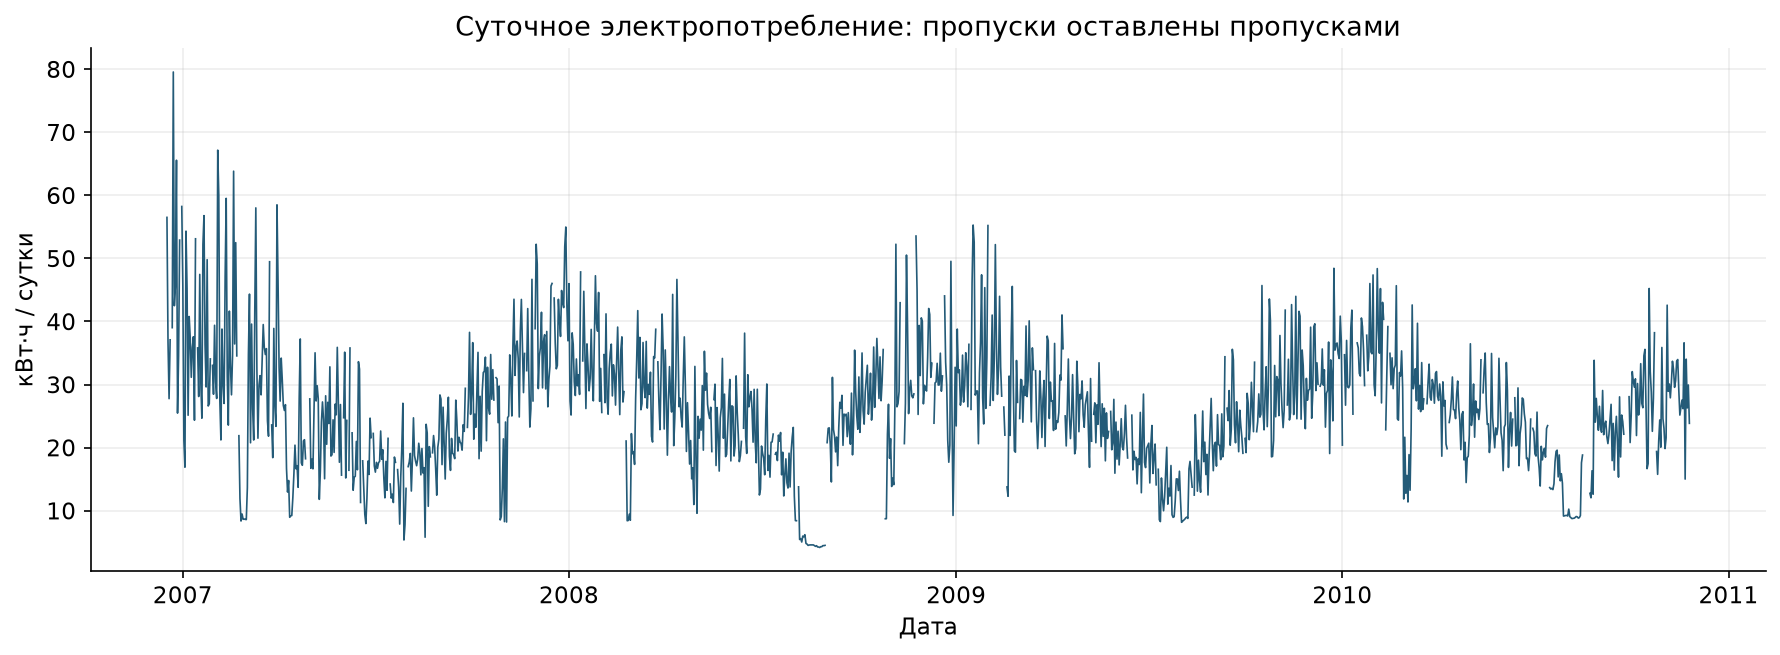
\includegraphics[width=\textwidth]{01_daily_energy.png}
 \caption{Исходный ряд суточного электропотребления. Разрывы соответствуют дням с неполными измерениями.}
 \label{fig:exp-daily-energy}
\end{figure}

Прогноз строится на один день вперёд. В признаки входят значения потребления с лагами $1$, $2$, $7$, $14$ и $28$ календарных дней; средние, стандартные отклонения и числа известных наблюдений за предыдущие $7$ и $28$ суток; семь индикаторов дня недели и два признака годового цикла:
\[
 \sin\left(\frac{2\pi(d_{\mathrm{year}}-1)}{365{,}25}\right),
 \qquad
 \cos\left(\frac{2\pi(d_{\mathrm{year}}-1)}{365{,}25}\right),
\]
где $d_{\mathrm{year}}$ --- номер дня в году. Все скользящие статистики вычисляются после сдвига ряда на один день; для недельного окна требуется не менее пяти известных значений, для окна длины $28$ дней --- не менее двадцати. Таким образом, используется $20$ признаков, доступных до раскрытия прогнозируемого исхода.

Строки с неизвестной целью или отсутствующими необходимыми признаками удаляются после построения признаков на полной календарной сетке. В результате остаётся $989$ наблюдений. Они разделены в хронологическом порядке на обучающую, калибровочную и тестовую части в пропорции $60\%/20\%/20\%$ (табл.~\ref{tab:exp-split}). Перемешивание наблюдений не применяется.

\begin{table}[htbp]
 \centering
 \caption{Хронологическое разделение доступных наблюдений.}
 \label{tab:exp-split}
 \begin{tabular}{@{}lrrr@{}}
  \toprule
  Назначение & Число дней & Начало & Конец\\
  \midrule
  Обучение экспертов & 593 & 17.01.2007 & 17.04.2009\\
  Выбор активности & 198 & 18.04.2009 & 29.01.2010\\
  Тестирование & 198 & 31.01.2010 & 25.11.2010\\
  \bottomrule
 \end{tabular}
\end{table}

В дальнейшем шаг $t$ означает очередной доступный тестовый день, поэтому $T=198$. Соседние шаги не обязательно соответствуют соседним календарным датам. При прогнозировании разрешено использовать уже наблюдённое потребление предыдущих дней, в том числе тестовых. Следовательно, проводится последовательное прогнозирование на один день, а не одновременный прогноз всего тестового периода из одной начальной даты.

\FloatBarrier
\subsection{Эксперты и правило специализации}

В качестве экспертов используются Ridge, Lasso, Bayesian Ridge, Random Forest и Gradient Boosting. Первые три метода являются линейными регрессионными моделями с различными способами регуляризации, последние два --- ансамблями деревьев решений. Модели реализованы средствами библиотеки scikit-learn. Для линейных методов стандартизация признаков включена в процедуру обучения и на каждом проверочном разбиении оценивается только по его обучающей части.

Гиперпараметры выбирались по средней несимметричной абсолютной потере, определённой ниже, на трёх последовательных разбиениях внутри первых $593$ наблюдений. Обучающая часть в этих разбиениях расширяется, а проверочные интервалы имеют одинаковую календарную длительность. Для Ridge перебирались коэффициенты регуляризации $\{0{,}1;1;10;100\}$, для Lasso --- $\{0{,}01;0{,}1;0{,}5;1\}$. У Random Forest сравнивались максимальная глубина $4$ и отсутствие ограничения глубины, а также минимальные размеры листа $3$ и $10$. У Gradient Boosting перебирались скорости обучения $0{,}03$ и $0{,}07$ и глубины деревьев $2$ и $3$. Оба ансамбля содержат по $150$ деревьев; начальное значение генератора случайных чисел равно $42$.

Выбраны Ridge с коэффициентом $100$, Lasso с коэффициентом $0{,}5$, Random Forest без ограничения глубины с минимальным размером листа $10$ и Gradient Boosting со скоростью обучения $0{,}03$ и глубиной $2$. Bayesian Ridge использован с одной конфигурацией без перебора гиперпараметров. После выбора настроек каждый эксперт обучается на всей обучающей части и в ходе тестирования не переобучается. Отрицательные прогнозы заменяются нулём как при подборе параметров, так и при последующем прогнозировании.

Для каждого дня недели на калибровочной части вычисляются средние потери пяти экспертов. Три эксперта с наименьшими потерями объявляются активными в соответствующий день недели на всём тестовом периоде. Число активных экспертов фиксировано: $|E_t|=3$. При равенстве потерь используется порядок перечисления моделей. Поскольку день недели известен заранее, множество $E_t$ определяется до наблюдения $y_t$.

Полученное правило показано на рис.~\ref{fig:exp-activity}. Lasso активен во все дни; Ridge --- во вторник, среду, пятницу, субботу и воскресенье; Bayesian Ridge --- во вторник, субботу и воскресенье; Random Forest --- в понедельник и четверг; Gradient Boosting --- в понедельник, среду, четверг и пятницу. На тесте это даёт соответственно $198$, $136$, $69$, $62$ и $129$ активных шагов. Для сравнения на всём горизонте прогнозы спящих экспертов также сохраняются, однако их фактические потери не участвуют в обновлении sAdaHedge: при сне используется виртуальная потеря $m_t$.

\begin{figure}[htbp]
 \centering
 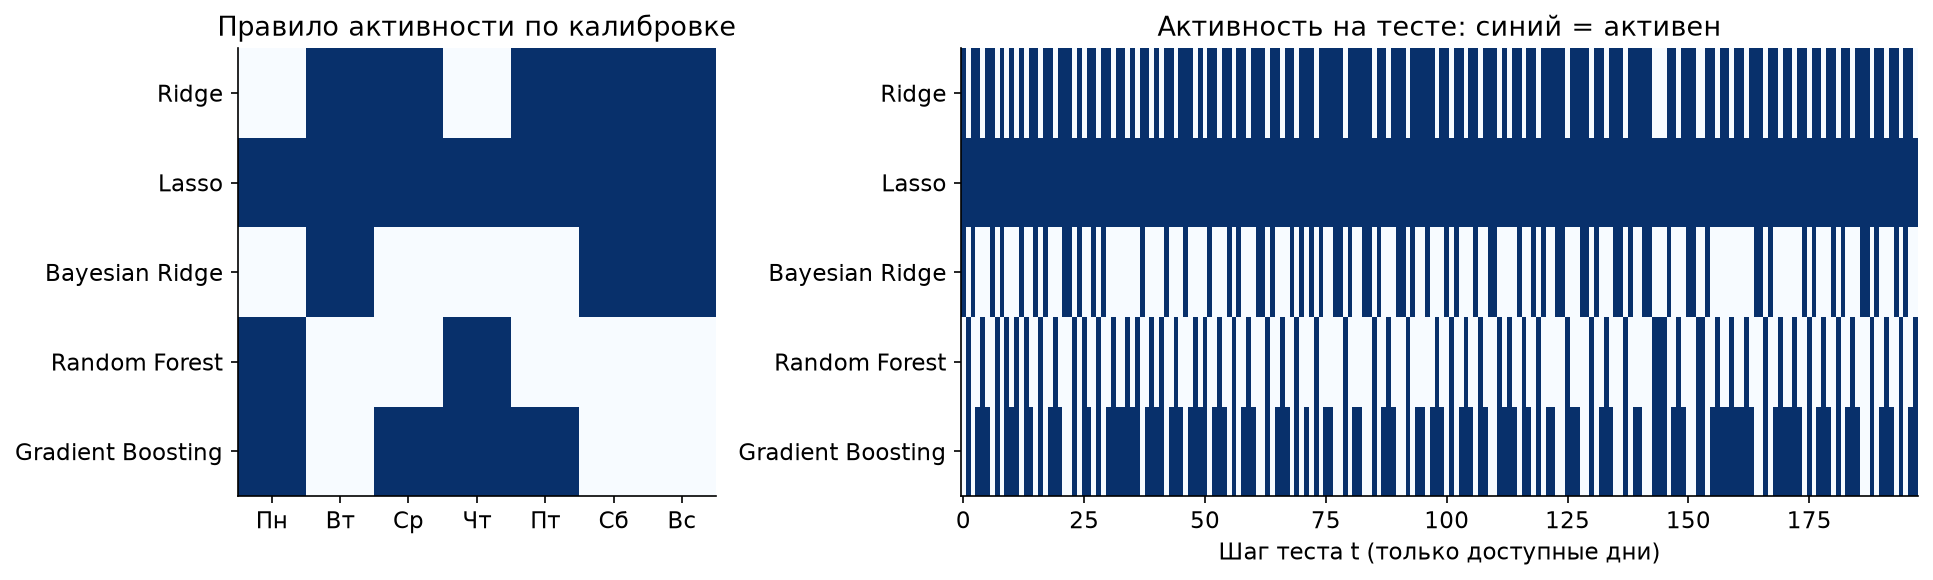
\includegraphics[width=\textwidth]{02_expert_activity.png}
 \caption{Специализация экспертов: правило активности по дням недели (слева) и его применение на тесте (справа). Синим отмечена активность. На правой панели доступные дни пронумерованы с нуля.}
 \label{fig:exp-activity}
\end{figure}

\FloatBarrier
\subsection{Функция потерь и протокол сравнения}

Для вычисления потерь потребление и прогнозы делятся на максимум целевой переменной обучающей части
\[
 C=67{,}16203\ \text{кВт}\cdot\text{ч}.
\]
Если $Y_t$ и $\widehat Y_t^i$ обозначают исход и прогноз эксперта в физических единицах, то в алгоритм передаются $y_t=Y_t/C$ и $\gamma_t^i=\widehat Y_t^i/C$. Масштаб $C$ не использует калибровочные или тестовые исходы; значения выше $C$ не обрезаются. Такая нормировка задаёт единицы измерения потерь, но не гарантирует принадлежности всех будущих значений интервалу $[0,1]$.

Используется выпуклая несимметричная абсолютная потеря
\begin{equation}
 \label{eq:exp-loss}
 \ell(\gamma,y)=|\gamma-y|_++2|y-\gamma|_+,
 \qquad |x|_+=\max\{x,0\}.
\end{equation}
Недооценка потребления штрафуется вдвое сильнее переоценки той же величины. Коэффициенты $\lambda_1=1$, $\lambda_2=2$ задают выбранный критерий сравнения и не интерпретируются как тарифы поставщика электроэнергии.

В начале теста агрегатор запускается с равномерными начальными весами, $L_0^i=0$ и $\Delta_0=0$. На каждом шаге он получает прогнозы активных экспертов, вычисляет веса по предыдущим потерям и выдаёт
\[
 \gamma_t=\sum_{i\in E_t}p_t^{i,E_t}\gamma_t^i.
\]
Только после раскрытия $y_t$ вычисляются потери и обновляется состояние алгоритма. Калибровочная часть используется для выбора активности и не входит в начальные кумулятивные потери агрегатора.

Сравниваются пять отдельных экспертов, sAdaHedge и два контрольных прогноза:
\[
 \gamma_t^{\mathrm{act}}=\frac1{|E_t|}\sum_{i\in E_t}\gamma_t^i,
 \qquad
 \gamma_t^{\mathrm{all}}=\frac1N\sum_{i=1}^{N}\gamma_t^i.
\]
Первый усредняет активных экспертов, второй --- всех пятерых. Для каждого метода на одних и тех же $198$ днях подсчитывается суммарная потеря~\eqref{eq:exp-loss}, а также средняя абсолютная ошибка и корень из средней квадратичной ошибки в физических единицах:
\[
 \operatorname{MAE}=\frac1T\sum_{t=1}^{T}|\widehat Y_t-Y_t|,
 \qquad
 \operatorname{RMSE}=\sqrt{\frac1T\sum_{t=1}^{T}(\widehat Y_t-Y_t)^2}.
\]
Здесь $\widehat Y_t=C\gamma_t$ для агрегатора; для остальных методов используется их соответствующий прогноз.

Будем различать фактические кумулятивные потери прогноза
\[
 A_T:=\sum_{t=1}^{T}\ell(\gamma_t,y_t)
\]
и кумулятивную смесь потерь $H_T=\sum_{t=1}^{T}\ell_t$. По выпуклости $A_T\leqslant H_T$, но эти величины в общем случае не совпадают. В таблицах качества приведены фактические потери прогнозов, тогда как при проверке теоретической оценки отдельно учитывается смесь.

\subsection{Качество прогнозирования на тестовом периоде}

На рис.~\ref{fig:exp-forecasts} приведены наблюдения и прогнозы для последних $90$ доступных тестовых дней. Прогноз sAdaHedge следует изменениям общего уровня потребления, однако, как и прогнозы отдельных экспертов, сглаживает часть резких суточных скачков. Особенно заметны недооценённые пики осенью и переоценка ряда низких значений в августе. Разрывы линий соответствуют исключённым дням, а не нулевым прогнозам.

\begin{figure}[htbp]
 \centering
 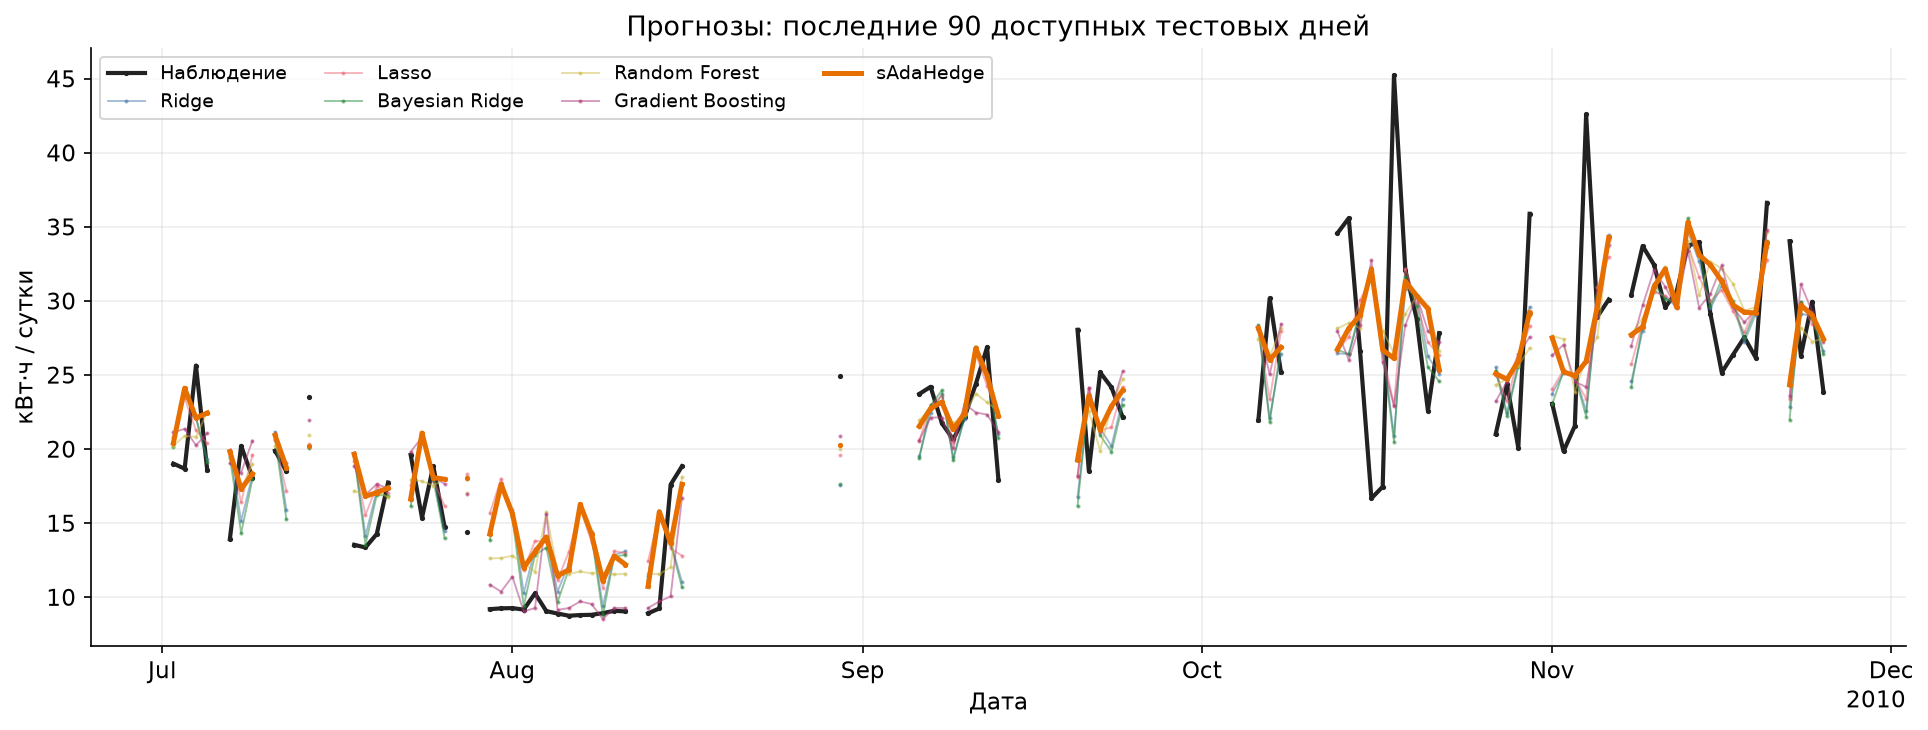
\includegraphics[width=\textwidth]{03_forecasts.png}
 \caption{Наблюдаемое потребление, прогнозы пяти экспертов и sAdaHedge на последних $90$ доступных днях теста. Значения приведены в кВт$\cdot$ч.}
 \label{fig:exp-forecasts}
\end{figure}

Итоговые показатели представлены в табл.~\ref{tab:exp-metrics}; методы упорядочены по суммарной несимметричной потере. Лучший результат по этому критерию имеет Random Forest: $17{,}23283$. Для sAdaHedge получено $17{,}46011$, что на $0{,}22728$, или приблизительно на $1{,}32\%$, больше. При этом sAdaHedge превосходит остальных четырёх экспертов и оба равномерных усреднения по выбранной потере. Преимущество над средним активных экспертов невелико: $0{,}07780$, или около $0{,}44\%$.

\begin{table}[htbp]
 \centering
 \caption{Качество прогнозов на всём тестовом горизонте ($T=198$). Потери вычислены после нормировки; MAE и RMSE --- в кВт$\cdot$ч.}
 \label{tab:exp-metrics}
 \begin{tabular}{@{}lrrr@{}}
  \toprule
  Метод & Суммарная потеря & MAE & RMSE\\
  \midrule
  Random Forest & $17{,}23283$ & $3{,}97616$ & $5{,}25696$\\
  sAdaHedge & $17{,}46011$ & $4{,}08681$ & $5{,}42988$\\
  Среднее активных & $17{,}53792$ & $4{,}05079$ & $5{,}41996$\\
  Gradient Boosting & $17{,}57012$ & $3{,}85351$ & $5{,}33035$\\
  Среднее всех & $17{,}88205$ & $4{,}01153$ & $5{,}44192$\\
  Lasso & $18{,}37446$ & $4{,}18644$ & $5{,}60173$\\
  Ridge & $18{,}83564$ & $4{,}19493$ & $5{,}74170$\\
  Bayesian Ridge & $19{,}02995$ & $4{,}21581$ & $5{,}80568$\\
  \bottomrule
 \end{tabular}
\end{table}

Ранжирование зависит от метрики. Наименьшая MAE достигается у Gradient Boosting ($3{,}85351$~кВт$\cdot$ч), а наименьшая RMSE --- у Random Forest ($5{,}25696$~кВт$\cdot$ч). Агрегатор не превосходит среднее активных экспертов по MAE и RMSE, несмотря на меньшую несимметричную потерю. Это согласуется с тем, что критерий~\eqref{eq:exp-loss} по-разному учитывает ошибки недооценки и переоценки.

Динамика кумулятивных потерь показана на рис.~\ref{fig:exp-cumulative}. В конце теста фактическая потеря агрегатора равна $A_T=17{,}46011$, а смесь потерь --- $H_T=17{,}50171$. Разность $H_T-A_T=0{,}04160$ соответствует выигрышу от усреднения прогнозов при выпуклой функции потерь. Кривые близки, поэтому на графике сплошная и пунктирная линии агрегатора почти совпадают.

\begin{figure}[htbp]
 \centering
 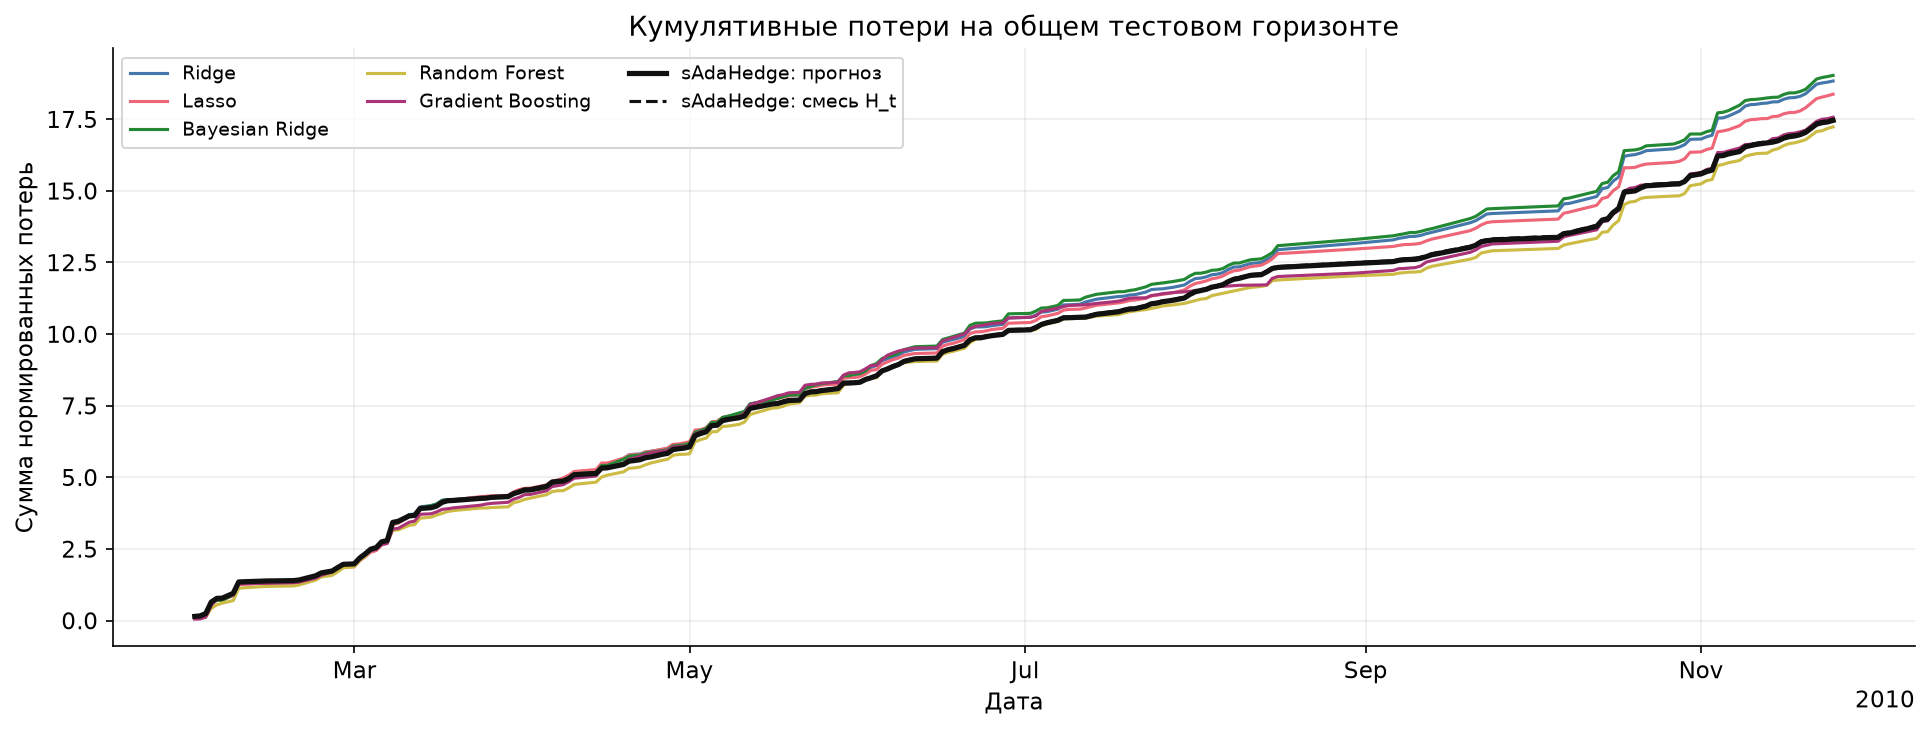
\includegraphics[width=\textwidth]{04_cumulative_losses.png}
 \caption{Кумулятивные фактические потери экспертов и sAdaHedge на всём тесте. Чёрный пунктир показывает смесь потерь $H_t$, чёрная сплошная линия --- потери прогнозов $A_t$.}
 \label{fig:exp-cumulative}
\end{figure}

\FloatBarrier
\subsection{Регрет на активных шагах и теоретическая граница}

На днях активности каждого эксперта наряду с регретом смеси $\widetilde R_T^i$ из~\eqref{eq:specialist-regret} вычислим регрет фактического прогноза:
\[
 \widetilde R_{T,\mathrm{pred}}^i
 :=\sum_{\substack{1\leqslant t\leqslant T\\i\in E_t}}
 \bigl(\ell(\gamma_t,y_t)-\ell(\gamma_t^i,y_t)\bigr).
\]
Отрицательное значение означает, что на этих днях агрегатор понёс меньшие потери, чем эксперт. Результаты приведены в табл.~\ref{tab:exp-specialist}.

\begin{table}[htbp]
 \centering
 \caption{Сравнение на днях активности каждого эксперта. $\mathcal L_T^i$ --- фактические потери эксперта на этих днях.}
 \label{tab:exp-specialist}
 \begin{tabular}{@{}lrrrr@{}}
  \toprule
  Эксперт & Активных дней & $\mathcal L_T^i$ & $\widetilde R_{T,\mathrm{pred}}^i$ & $\widetilde R_T^i$\\
  \midrule
  Ridge & 136 & $11{,}07508$ & $-0{,}01726$ & $-0{,}00878$\\
  Lasso & 198 & $18{,}37446$ & $-0{,}91434$ & $-0{,}87275$\\
  Bayesian Ridge & 69 & $6{,}37518$ & $0{,}07206$ & $0{,}07270$\\
  Random Forest & 62 & $6{,}22361$ & $0{,}17868$ & $0{,}21180$\\
  Gradient Boosting & 129 & $11{,}06780$ & $-0{,}05492$ & $-0{,}01397$\\
  \bottomrule
 \end{tabular}
\end{table}

Регрет отрицателен для Ridge, Lasso и Gradient Boosting и положителен для Bayesian Ridge и Random Forest. Наибольший регрет смеси --- $0{,}21180$ относительно Random Forest. В конце теста получены
\[
 V_T\approx0{,}02273,\qquad S_T\approx0{,}22454,
 \qquad 2\Delta_T\approx0{,}43265,
\]
а правая часть теоретической оценки при $N=5$ равна
\[
 B_T:=2\sqrt{V_T\ln5}+S_T\left(\frac43\ln5+2\right)
 \approx1{,}31346.
\]
Все регреты специалистов меньше $2\Delta_T$ и $B_T$; дисперсионная граница заметно превышает наблюдаемые значения.

По сохранённой последовательности вычислений для каждого префикса $t=1,\dots,T$ и каждого эксперта проверена цепочка
\[
 \widetilde R_{t,\mathrm{pred}}^i
 \leqslant\widetilde R_t^i
 \leqslant H_t-L_t^i
 \leqslant2\Delta_t
 \leqslant B_t
\]
с численным допуском $10^{-9}$; нарушений не обнаружено. Расширенные потери $L_t^i$ включают виртуальные потери во время сна.

\begin{figure}[htbp]
 \centering
 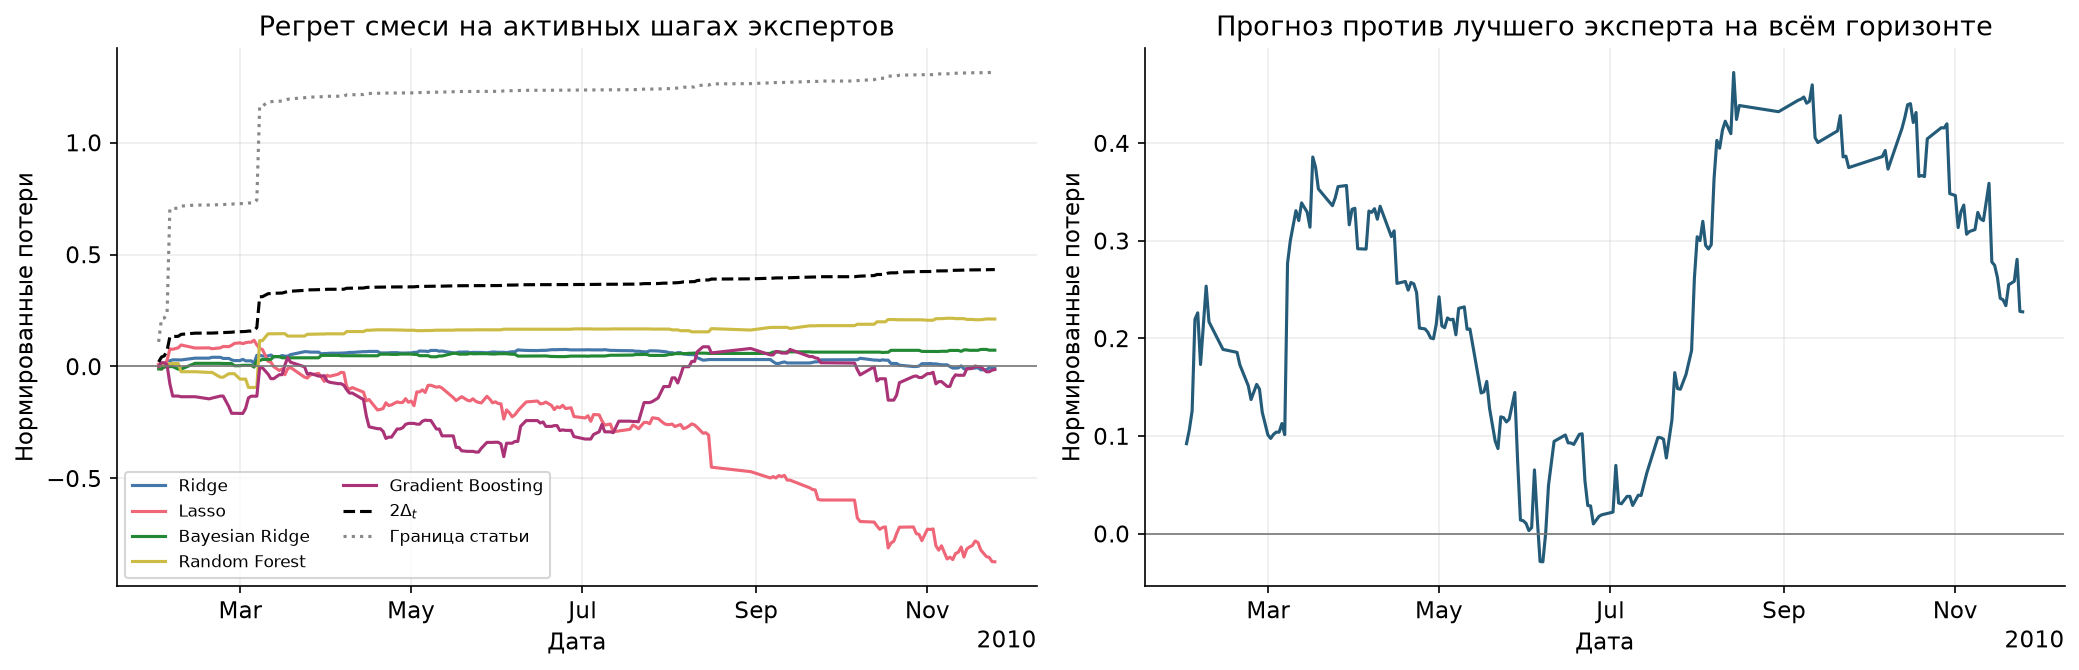
\includegraphics[width=\textwidth]{05_regret_and_bound.png}
 \caption{Слева: регрет смеси относительно специалистов, граница $2\Delta_t$ и дисперсионная граница $B_t$. Справа: регрет фактического прогноза относительно лучшего фиксированного эксперта на каждом полном префиксе теста.}
 \label{fig:exp-regret}
\end{figure}

Левая панель рис.~\ref{fig:exp-regret} показывает регрет на активных шагах. На правой панели приведён другой критерий:
\[
 R_{t,\mathrm{full}}
 :=A_t-\min_{i\in I}\sum_{s=1}^{t}\ell(\gamma_s^i,y_s),
\]
где для каждого эксперта учитываются все тестовые дни, включая дни его сна. Минимум берётся отдельно на каждом префиксе; эксперт, достигающий минимума, может меняться с $t$. При $t=T$ получаем $R_{T,\mathrm{full}}=0{,}22728$. Оценка~\eqref{eq:specialist-regret-bound} непосредственно относится к сравнению на активных шагах и не даёт такой же гарантии для $R_{t,\mathrm{full}}$.

Попарные кумулятивные сравнения представлены на рис.~\ref{fig:exp-active-comparison}. В пределах каждой панели все три суммы вычислены по одним и тем же дням активности соответствующего эксперта. Между панелями наборы дней и их количество различаются, поэтому сами величины кумулятивных потерь на разных панелях не служат основанием для ранжирования экспертов.

\begin{figure}[htbp]
 \centering
 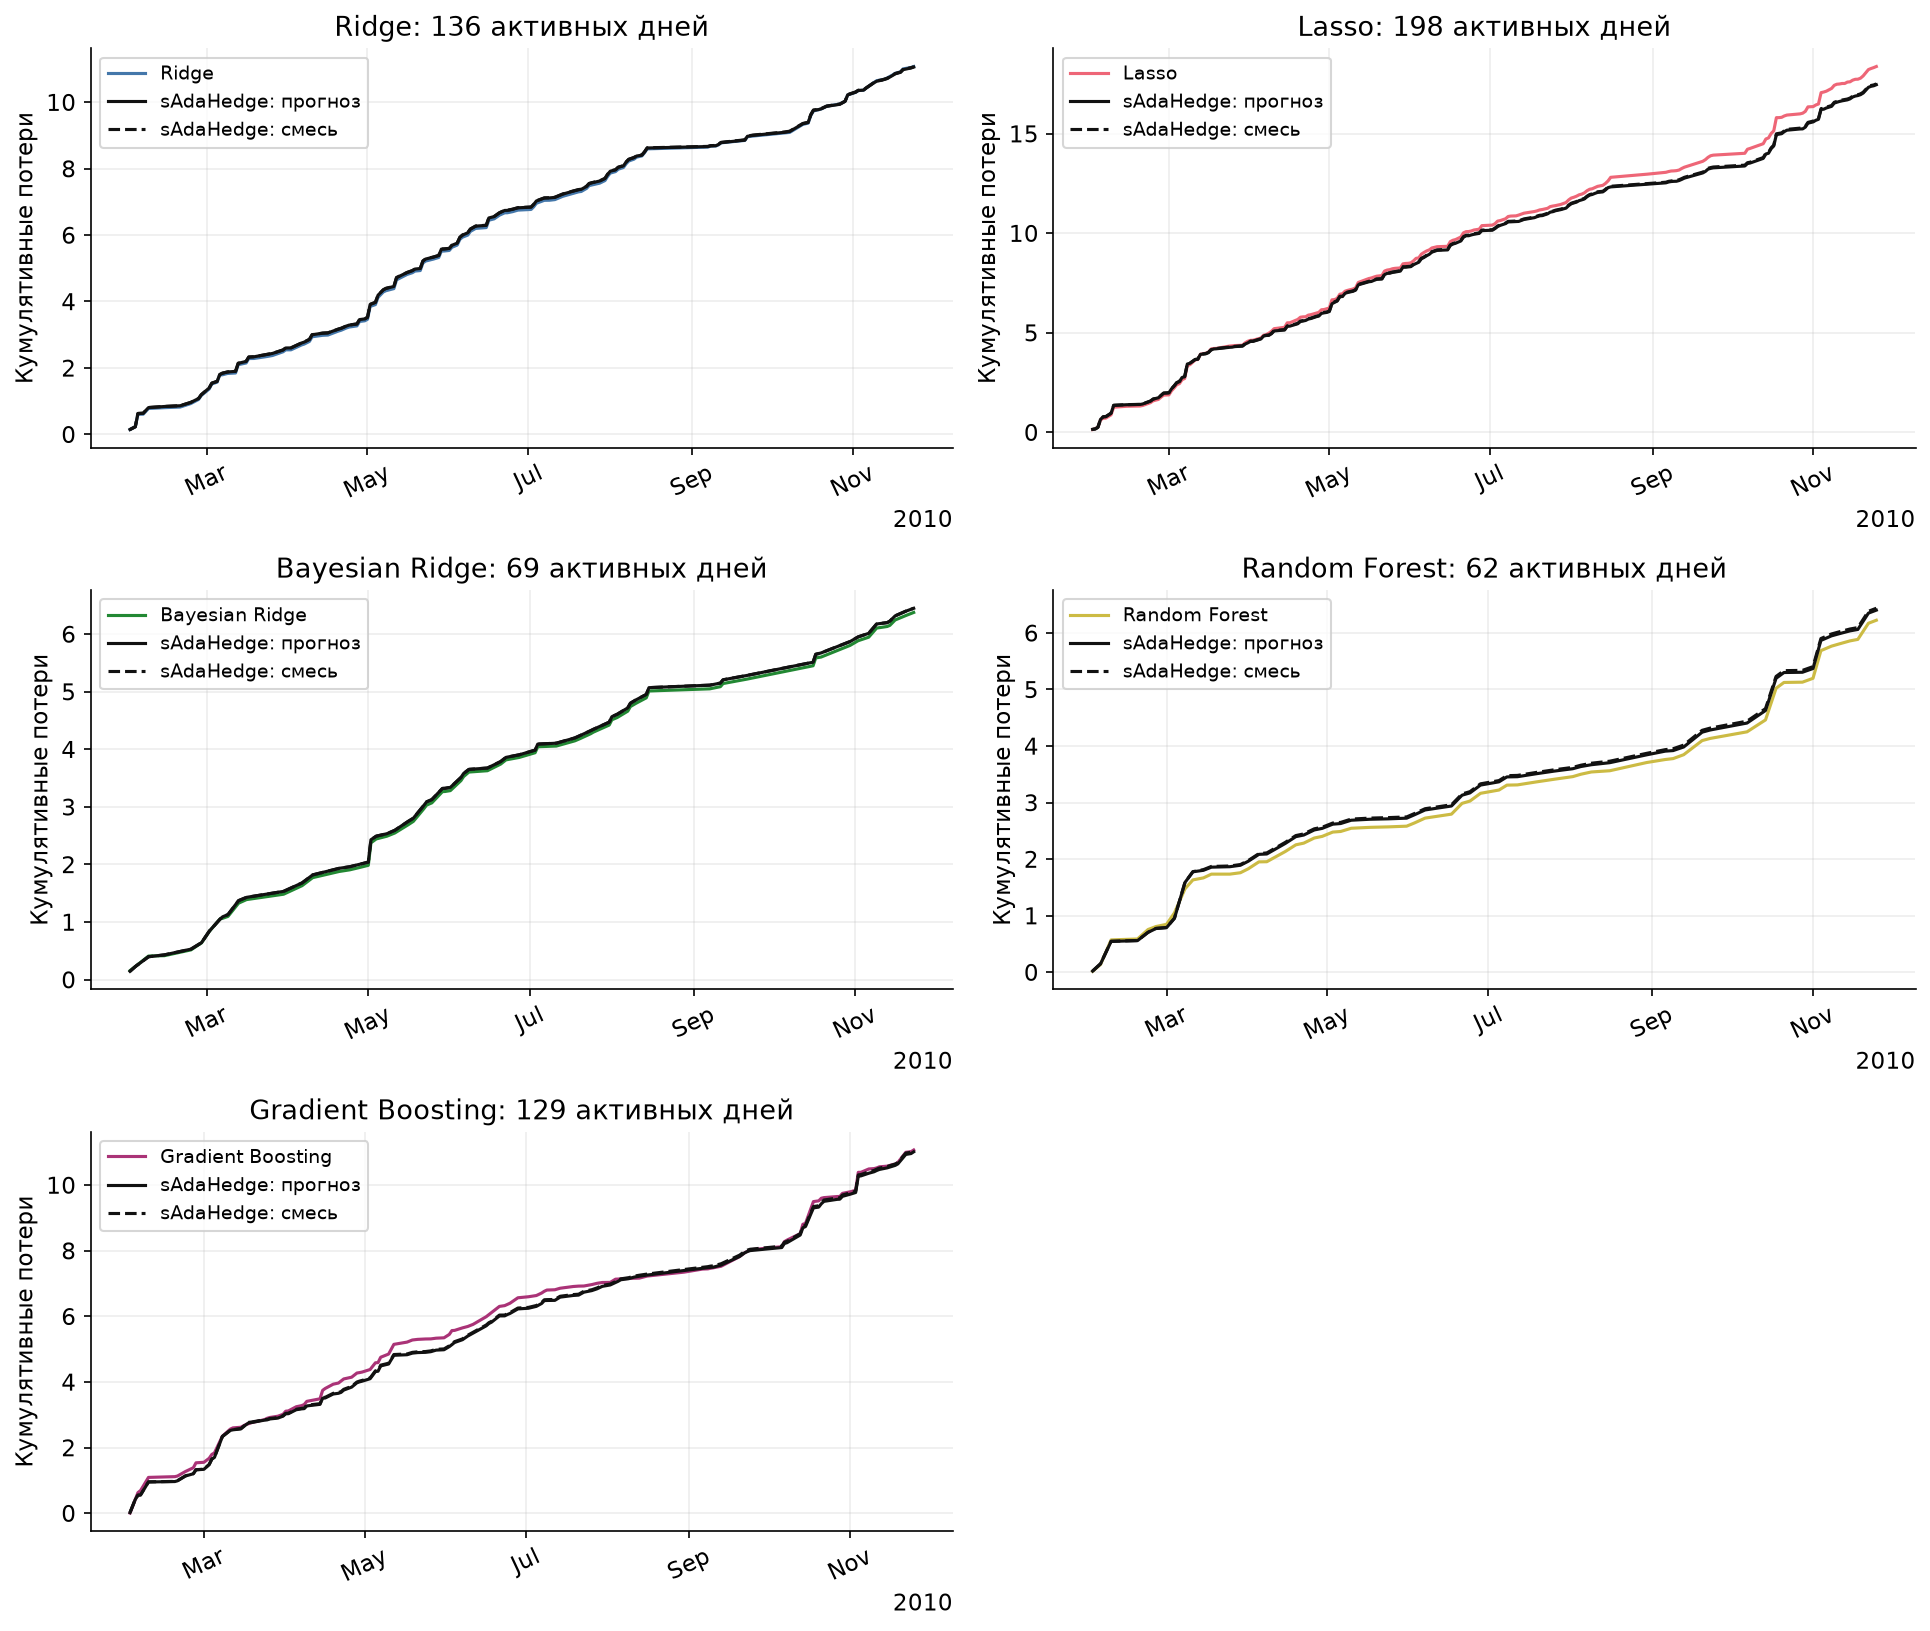
\includegraphics[width=\textwidth,height=0.68\textheight,keepaspectratio]{06_active_only_comparisons.png}
 \caption{Попарные сравнения на активных шагах: потери эксперта, фактические потери sAdaHedge и смесь потерь агрегатора. На каждой панели используется собственное множество дней.}
 \label{fig:exp-active-comparison}
\end{figure}

\FloatBarrier
\subsection{Динамика весов и выводы}

На рис.~\ref{fig:exp-weights} показаны веса активных экспертов и параметр обучения. Для изображения вес спящего эксперта принимается равным нулю. Поэтому часть резких изменений верхних кривых связана с календарным переключением множества $E_t$ и последующей нормировкой весов. Нулевой вес во время сна не означает удаления эксперта: при следующей активации он снова участвует в прогнозе.

\begin{figure}[htbp]
 \centering
 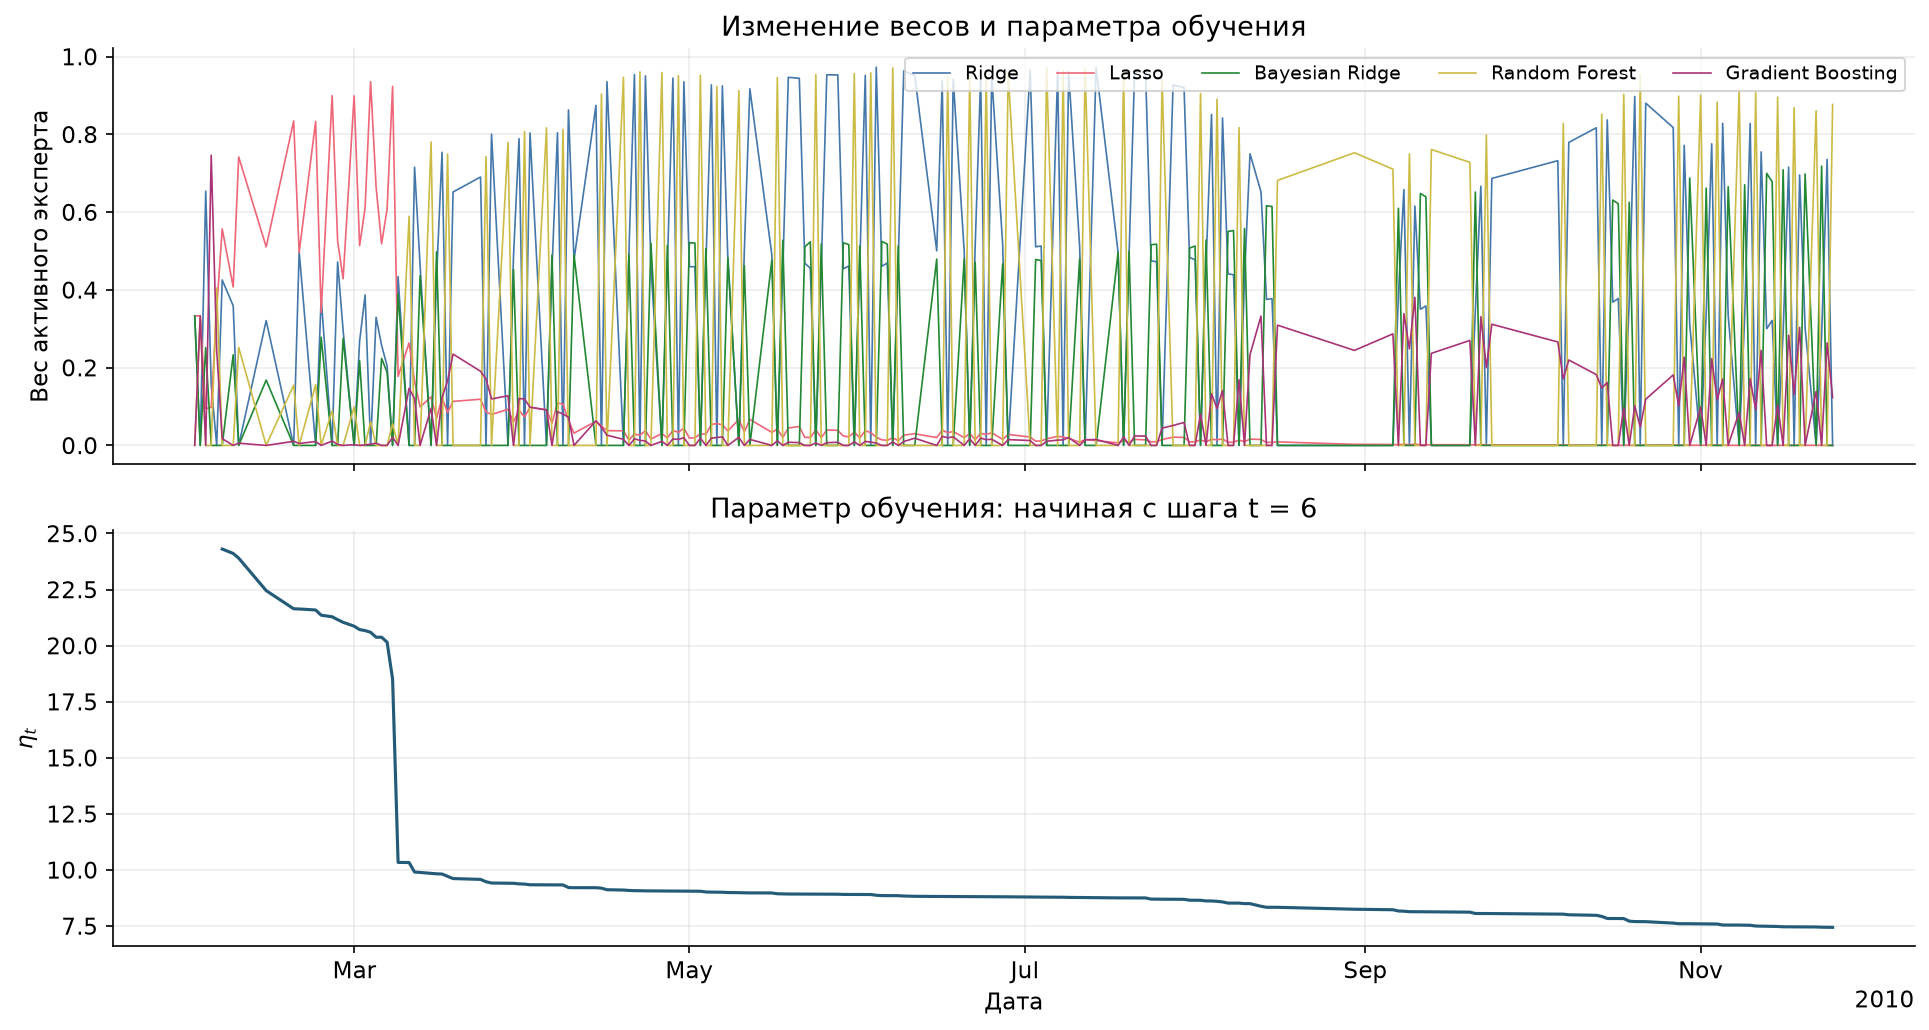
\includegraphics[width=\textwidth]{07_weights_and_eta.png}
 \caption{Веса экспертов в прогнозе sAdaHedge (сверху) и параметр обучения $\eta_t$ (снизу). Нижняя панель начинается с шестого шага; первые пять значений исключены только из изображения.}
 \label{fig:exp-weights}
\end{figure}

В начале теста заметную долю веса получает Lasso; далее в соответствующие дни активности существенный вес часто приходится на Ridge и Random Forest. Параметр $\eta_t$ не возрастает, поскольку $\Delta_t$ не убывает. На первом шаге используется соглашение $\eta_1=\infty$; уже на втором шаге параметр конечен и равен приблизительно $161{,}60$. Для читаемости на нижней панели показана последовательность начиная с $t=6$, когда $\eta_6\approx24{,}31$. К последнему шагу параметр снижается до $\eta_T\approx7{,}44$.

В проведённом эксперименте sAdaHedge даёт близкое к лучшему фиксированному эксперту качество по несимметричной потере и небольшое преимущество над равномерным усреднением активных прогнозов. На активных шагах трёх из пяти экспертов регрет отрицателен; для двух остальных он положителен и остаётся в пределах теоретической оценки. При этом на всём тестовом горизонте лучшим по выбранной потере оказался Random Forest, активный в агрегаторе лишь два дня недели. Следовательно, качество фиксированного правила специализации существенно для интерпретации общего результата.

Выводы относятся к одному временному ряду, одному хронологическому разбиению и выбранным коэффициентам потерь. Небольшое преимущество перед равномерным усреднением здесь является наблюдаемым результатом; статистическая значимость этого различия не оценивалась. Дальнейшее сравнение может включать несколько последовательных тестовых периодов, другие числа активных экспертов и чувствительность к отношению $\lambda_2/\lambda_1$.

\FloatBarrier

\section{Заключение}
\label{sec:conclusion}

В работе рассмотрена задача последовательного прогнозирования с советами экспертов и её обобщение на экспертов-специалистов, участвующих в прогнозе лишь на части шагов. Изложены экспоненциальное смешивание потерь, адаптивный выбор параметра обучения и алгоритм sAdaHedge. Приведено доказательство оценки его регрета относительно каждого специалиста через накопленную дисперсию и максимальный размах потерь активных экспертов. Показано, что при выпуклой функции потерь эта оценка переносится со смеси потерь на фактические потери усреднённого прогноза.

Численный эксперимент на суточном электропотреблении продемонстрировал применение схемы с пятью регрессионными экспертами и специализацией по дням недели. На $198$ тестовых днях суммарная нормированная потеря sAdaHedge составила $17{,}46011$, у лучшего фиксированного эксперта Random Forest --- $17{,}23283$, а у равномерного среднего активных экспертов --- $17{,}53792$. Следовательно, адаптивное взвешивание дало небольшое улучшение по сравнению с равномерным смешиванием, но не обеспечило превосходства над лучшим отдельным методом на всём горизонте. На днях активности трёх из пяти экспертов регрет агрегатора оказался отрицательным; теоретические неравенства для специалистов выполнены на каждом префиксе тестовой последовательности.

Полученные результаты выделяют два компонента качества: сами прогнозы экспертов и правило их допуска к агрегированию. Адаптация весов позволяет использовать различия в качестве доступных прогнозов, однако не исправляет автоматически неудачный выбор множества активных экспертов. Кроме того, адаптивный параметр обучения не означает забывания прошлых потерь: в рассмотренной схеме они накапливаются за всё время работы. Эти особенности определяют дальнейшие направления исследования.

\subsection*{Открытые вопросы и направления продолжения}

Следующие вопросы остаются открытыми в рамках проведённого исследования. Предлагаемые изменения требуют отдельных вычислительных экспериментов, а при изменении алгоритма --- проверки условий и доказательства соответствующих гарантий.

\begin{enumerate}
 \item \textbf{Как выбирать и обновлять специализацию?}
 В эксперименте активность один раз определяется по калибровочной выборке и зависит только от дня недели. Можно пересматривать её по скользящему окну прошлых ошибок, учитывать сезон, праздники и доступный на момент прогноза прогноз погоды. Следует сравнить разные числа активных экспертов, включая вариант $E_t=I$, и проверить, даёт ли специализация выигрыш по сравнению с агрегированием всех пяти моделей. При сохранении протокола sAdaHedge множество $E_t$ должно оставаться непустым и определяться до раскрытия $y_t$. Сама оценка относительно выбранных специалистов не гарантирует высокого качества правила, которое выбирает их активность; оценивание и обучение этого правила составляют отдельную задачу.

 \item \textbf{Как ускорить адаптацию к смене режима ряда?}
 Если лучший эксперт меняется со временем, старые потери могут долго влиять на его вес. Возможные модификации --- скользящее окно потерь, их дисконтирование, перезапуски агрегатора и небольшое перераспределение веса между экспертами. Для оценки таких изменений целесообразно перейти от всего горизонта к сравнению на отрезках, связанному с постановкой адаптивного регрета~\cite{Adaptive}. В случае специалистов естественен критерий
 \[
  \widetilde R_{[a,b],\mathrm{pred}}^i
  :=\sum_{\substack{a\leqslant t\leqslant b\\i\in E_t}}
  \bigl(\ell(\gamma_t,y_t)-\ell(\gamma_t^i,y_t)\bigr).
 \]
 Вопрос состоит в том, какие гарантии можно получить для него одновременно на разных временных отрезках и какова цена быстрой адаптации. Оценка на полном горизонте сама по себе этого не устанавливает; замена накопленных потерь оконными или дисконтированными требует нового анализа.

 \item \textbf{Можно ли заменить бинарную активность степенью участия?}
 Вместо решения <<активен или спит>> можно задавать до наблюдения исхода коэффициент $c_t^i\in[0,1]$, отражающий пригодность эксперта для текущего контекста. Это позволяет исследовать плавный переход между режимами и уменьшить зависимость от жёсткого выбора трёх лучших моделей. Необходимо согласовать правило взвешивания с критерием качества, например с регретом
 \[
  \sum_{t=1}^{T}c_t^i
  \bigl(\ell(\gamma_t,y_t)-\ell(\gamma_t^i,y_t)\bigr),
 \]
 и определить соответствующие виртуальные потери. Простая замена индикатора активности на $c_t^i$ в итоговой оценке без изменения доказательства недостаточна.

 \item \textbf{Как улучшить и разнообразить исходные прогнозы?}
 Сейчас все эксперты используют один набор признаков и после обучения остаются неизменными. Можно добавить сезонный прогноз по значению неделю назад, модели с разной длиной обучающего окна и экспертов, специализирующихся на высоком или низком уровне потребления. Полезно сравнить периодическое переобучение с фиксированными моделями и согласовать обучение экспертов с несимметричной функцией потерь, которая используется для итоговой оценки. При этом обновлённая модель должна получать только уже раскрытые исходы. Основной вопрос --- даёт ли расширение набора экспертов полезное разнообразие ошибок и компенсирует ли улучшение качества дополнительные вычислительные затраты.

 \item \textbf{Насколько можно уточнить оценку регрета?}
 В эксперименте наибольший регрет смеси равен примерно $0{,}21180$, промежуточная граница $2\Delta_T$ --- $0{,}43265$, а дисперсионная граница --- $1{,}31346$. Это мотивирует поиск более точных оценок для отдельных экспертов. Представляет интерес зависимость от числа их активных шагов и характеристик потерь именно на этих шагах, особенно для редко активных специалистов. Такая локализация не следует простой заменой $V_T$ и $S_T$ в доказанной формуле: состояние агрегатора меняется и во время сна рассматриваемого эксперта. Возможное продолжение включает как вывод уточнённой оценки, так и построение примеров, показывающих ограничения такого уточнения.

 \item \textbf{Насколько устойчивы экспериментальные выводы?}
 Следует повторить сравнение на нескольких хронологических разбиениях и других рядах потребления, исследовать разные отношения $\lambda_2/\lambda_1$, число активных экспертов и длину калибровочного периода. Для отделения вклада компонентов нужны варианты с одинаковыми прогнозами экспертов, но разными правилами активности и взвешивания. Сравнение ошибок следует проводить по совпадающим дням и учитывать их временную зависимость при оценке неопределённости. Отдельно можно проверить влияние исключения неполных суток и сравнить его с причинным восстановлением недостающих признаков, сохраняя оценку качества на реально наблюдённых целевых значениях.
\end{enumerate}

\clearpage
\phantomsection
\addcontentsline{toc}{section}{\refname}
% Все записи ниже выводятся в списке литературы, даже если пока не процитированы.
% Ключи для \cite: CBL, FreundSchapire, VyuginSham, Adaptive, AdaHedge, Devaine.
% Новый источник добавляйте через \bibitem{УникальныйКлюч} перед
% \end{thebibliography}; затем ссылайтесь на него с помощью \cite.
\begin{thebibliography}{9}

\bibitem{CBL}
Cesa-Bianchi N., Lugosi G.
\emph{Prediction, Learning, and Games}.
Cambridge University Press, 2006.
\href{https://cesa-bianchi.di.unimi.it/predbook/}{Страница книги}.

\bibitem{FreundSchapire}
Freund Y., Schapire R.~E.
A decision-theoretic generalization of on-line learning and an application to boosting.
\emph{Journal of Computer and System Sciences}. 1997. Vol.~55, no.~1. P.~119--139.
\href{https://www.schapire.net/papers/FreundSc95.pdf}{Авторская версия}.

\bibitem{VyuginSham}
V'yugin V.~V., Shamsutdinov A.~I.
Trading-Network Order Formation with the Help of the Aggregation of Specialized Forecast Algorithms.
\emph{Journal of Communications Technology and Electronics}. 2016. Vol.~61. P.~1400--1410.
\url{https://doi.org/10.1134/S1064226916120251}.

\bibitem{Adaptive}
Adamskiy D., Koolen W.~M., Chernov A., Vovk V.
A Closer Look at Adaptive Regret.
\emph{Journal of Machine Learning Research}. 2016. Vol.~17, no.~23. P.~1--21.
\url{https://www.jmlr.org/papers/v17/13-533.html}.

\bibitem{AdaHedge}
De Rooij S., Van Erven T., Gr\"unwald P.~D., Koolen W.~M.
Follow the Leader If You Can, Hedge If You Must.
\emph{Journal of Machine Learning Research}. 2014. Vol.~15, no.~37. P.~1281--1316.
\url{https://www.jmlr.org/papers/v15/rooij14a.html}.

\bibitem{Devaine}
Devaine M., Gaillard P., Goude Y., Stoltz G.
Forecasting electricity consumption by aggregating specialized experts.
\emph{Machine Learning}. 2013. Vol.~90, no.~2. P.~231--260.
\url{https://doi.org/10.1007/s10994-012-5314-7}.

\bibitem{UCIHousehold}
Hebrail G., Berard A.
\emph{Individual Household Electric Power Consumption} [набор данных].
UCI Machine Learning Repository, 2006.
\url{https://doi.org/10.24432/C58K54}.

\end{thebibliography}

\end{document}
